%% USEFUL LINKS:
%% -------------
%%
%% - UiO LaTeX guides:          https://www.mn.uio.no/ifi/tjenester/it/hjelp/latex/
%% - Mathematics:               https://en.wikibooks.org/wiki/LaTeX/Mathematics
%% - Physics:                   https://ctan.uib.no/macros/latex/contrib/physics/physics.pdf
%% - Basics of Tikz:            https://en.wikibooks.org/wiki/LaTeX/PGF/Tikz
%% - All the colors!            https://en.wikibooks.org/wiki/LaTeX/Colors
%% - How to make tables:        https://en.wikibooks.org/wiki/LaTeX/Tables
%% - Code listing styles:       https://en.wikibooks.org/wiki/LaTeX/Source_Code_Listings
%% - \includegraphics           https://en.wikibooks.org/wiki/LaTeX/Importing_Graphics
%% - Learn more about figures:  https://en.wikibooks.org/wiki/LaTeX/Floats,_Figures_and_Captions
%% - Automagic bibliography:    https://en.wikibooks.org/wiki/LaTeX/Bibliography_Management  (this one is kinda difficult the first time)
%%
%%                              (This document is of class "revtex4-1", the REVTeX Guide explains how the class works)
%%   REVTeX Guide:              http://www.physics.csbsju.edu/370/papers/Journal_Style_Manuals/auguide4-1.pdf
%%
%% COMPILING THE .pdf FILE IN THE LINUX IN THE TERMINAL
%% ----------------------------------------------------
%%
%% [terminal]$ pdflatex report_example.tex
%%
%% Run the command twice, always.
%%
%% When using references, footnotes, etc. you should run the following chain of commands:
%%
%% [terminal]$ pdflatex report_example.tex
%% [terminal]$ bibtex report_example
%% [terminal]$ pdflatex report_example.tex
%% [terminal]$ pdflatex report_example.tex
%%
%% This series of commands can of course be gathered into a single-line command:
%% [terminal]$ pdflatex report_example.tex && bibtex report_example.aux && pdflatex report_example.tex && pdflatex report_example.tex
%%
%% ----------------------------------------------------

\PassOptionsToPackage{square,comma,numbers,sort&compress,super}{natbib}
\documentclass[aps,pra,english,notitlepage,reprint,nofootinbib]{revtex4-1}  % defines the basic parameters of the document
% For preview: skriv i terminal: latexmk -pdf -pvc filnavn
% If you want a single-column, remove "reprint"

% Allows special characters (including æøå)
% \usepackage[mathletters]{ucs}
% \usepackage[utf8x]{inputenc}
% \usepackage[english]{babel}
\usepackage{silence}
\WarningFilter{revtex4-1}{Repair the float}

%% Note that you may need to download some of these packages manually, it depends on your setup.
%% I recommend downloading TeXMaker, because it includes a large library of the most common packages.

\usepackage{physics,amssymb}  % mathematical symbols (physics imports amsmath)
\usepackage{amsmath}
\usepackage{graphicx}
% include graphics such as plots
\usepackage[dvipsnames]{xcolor}           % set colors
% \usepackage{hyperref}         % automagic cross-referencing
%\usepackage{url}
% \usepackage{cleveref}
\usepackage{listings}         % display code
\usepackage{subfigure}        % imports a lot of cool and useful figure commands
\usepackage{subcaption}
%\usepackage{float}
%\usepackage[section]{placeins}
\usepackage{algorithm}
\usepackage[noend]{algpseudocode}
\usepackage{cprotect}
\usepackage{multirow}
\usepackage{array, booktabs}
\newcolumntype{C}[1]{>{\centering\let\newline\\\arraybackslash\hspace{0pt}}m{#1}}
\usepackage[noend]{algpseudocode}
\usepackage{subfigure}
\newcommand{\imp}{\hspace{5pt}\Rightarrow\hspace{5pt}}
\newcommand\numberthis{\addtocounter{equation}{1}\tag{\theequation}}
\usepackage{tikz}
\usepackage{hyperref}         % automagic cross-referencing
\usepackage{cleveref}
\usepackage{comment}
% defines the color of hyperref objects
% Blending two colors:  blue!80!black  =  80% blue and 20% black
\hypersetup{ % this is just my personal choice, feel free to change things
    colorlinks,
    linkcolor={red!50!black},
    citecolor={blue!50!black},
    urlcolor={blue!80!black},
breaklinks=true}
\urlstyle{same}

\renewcommand{\bibsection}{\section*{References}}
\newcommand{\psp}{\hspace{1pt}}
% ===========================================

\begin{document}

\title{\texorpdfstring{
        \begin{Large}Project 2
\end{Large}\\\vspace{5pt}FYS-STK4155}{Lg}}
\author{Erik Joshua Røset \& Oskar Idland}
\date{\today}
\affiliation{University of Oslo, Department of Physics}

\begin{abstract}
    \centering
    In this project, we extend our exploration of machine learning techniques to include advanced optimization algorithms and neural networks. We implement and analyze gradient descent methods and feed-forward neural networks. With a focus on the vast hyperparameter space for these techniques, we systematically tune their values and analyze their influence on our models. We apply these methods to both regression and classification tasks, using synthetic data generated through the Franke function and the Wisconsin Breast Cancer dataset. Our neural network implementation achieves MSE values of $10^{-3}$ and $R^2$ scores above 0.99 for the Franke function regression. For the breast cancer classification task, our model attains 98.2\% test accuracy, demonstrating the effectiveness of our optimization approach. Our results demonstrate the importance of activation functions, initialization strategies, and regularization methods in training effective neural networks. We also highlight the impact of optimization techniques on model convergence and generalization, providing a comprehensive overview of the fundamental building blocks of modern machine learning systems..
\end{abstract}
\maketitle
\onecolumngrid
\begin{center}
    \vspace{-15pt}
    % LINK TO REPOSITORY
    \href{https://github.com/Oskar-Idland/FYS-STK4155-Projects}{https://github.com/Oskar-Idland/FYS-STK4155-Projects}%{GitHub Repository}
    \vspace{5pt}
\end{center}
\twocolumngrid
% ===========================================



\section{Introduction}\label{sec:introduction}

The rapid advancement of artificial intelligence (AI) and machine learning has significantly impacted various fields, with medical imaging and diagnostics being among the most benefited areas \cite{litjens2017survey}. A key development in this field is the use of Convolutional Neural Networks (CNNs), a type of deep learning model known for being effective in image recognition and classification. CNNs are widely used in healthcare, especially for important tasks like tumor detection and disease classification, where accuracy and efficiency are crucial \cite{9395920}. However, many traditional neural networks, including CNNs, need a lot of computational power, which can make them less suitable for use in resource-limited environments \cite{howard2017mobilenetsefficientconvolutionalneural}. 

To address this, more efficient architectures like MobileNet and ResNet have been created. MobileNet is designed to be lightweight and efficient, making it ideal for tasks like medical image classification \cite{howard2017mobilenetsefficientconvolutionalneural}. ResNet, on the other hand, uses residual connections to help train deep networks, which solves the degradation problem and improves performance in complex image recognition tasks \cite{he2015deepresiduallearningimage}. Together, these architectures offer a range of solutions for efficient and effective deep learning in medical imaging applications.

This study aims to evaluate and compare the performance of various neural network architectures on a breast cancer histopathological dataset, focusing on three specific models: a custom CNN, MobileNet, and ResNet101. These models are selected based on their differing complexities, training requirements, and computational efficiencies. In this analysis, we will compare how well these models handle a small and imbalanced dataset, aiming to understand how different architectures affect classification accuracy and performance in medical applications.

This report is organized as follows: First, we introduce the theoretical concepts behind neural networks, CNNs, MobileNet, and ResNet, along with the relevant evaluation metrics. Next, we discuss the methods and implementation, including data preprocessing and model architectures. We then present the results, comparing the performance of the models. Finally, we conclude by summarizing our findings and identifying the most suitable model for handling complex data.

% In \cref{sec:theory} we present relevant background theory, the majority of which has been sourced from the lecture notes by Morten Hjorth-Jensen \cite{notes}. We go into detail explaining central concepts such as OLS, Ridge and Lasso regression, the bias-variance tradeoff and two crucial resampling methods; bootstrapping and cross-validation, both of which will be implemented in this work. A few of the most important expressions introduced in this section are derived in \cref{appsec:derivations}. Our methodology is explained in \cref{sec:methods}, specifically how we define the essential design matrix, scale our data and implement the regression and resampling techniques. We also give an overview of our code structure and present the cosmological simulation data. In \cref{sec:results discussion} we present, interpret and discuss the results of our analyses in light of expectations based on our previous knowledge of the implemented regression and resampling methods. In \cref{appsec:figures} we include some additional figures that are not essential to our discussions, yet still referred to in the aforementioned section because they are necessary in reasoning our choice of presented results. Lastly, we summarize and conclude the main findings of our work in \cref{sec:conclusion}, and provide some open questions for further exploration.

% ===========================================
\section{Theory}\label{sec:theory}

In this project, we extend our previous exploration of machine learning techniques into more advanced optimization algorithms and neural networks. Gradient descent methods, along with their various enhancements, are crucial in training neural networks, which are used to model complex, non-linear relationships. While the foundational principles of regression analysis and optimization were addressed in our previous report, here we focus specifically on gradient descent with and without momentum, and tuning methods such as decaying learning rates, AdaGrad, RMSprop, and ADAM. Additionally, the fundamentals of neural networks will be discussed, emphasizing their relevance to the current project.

\subsection{Gradient Descent Methods}

Gradient descent is a fundamental optimization algorithm used to minimize a cost function \( C(\beta) \), where \( \beta \) represents the model parameters. Unlike the closed-form solutions available for OLS and Ridge regression in Project 1, many modern machine learning models, particularly neural networks, require iterative optimization methods. The core principle of gradient descent is to iteratively update the parameters in the direction that minimizes the cost function. Given a cost function \( C(\beta) \) and current parameters \( \beta_t \) at iteration \(t\), the basic update rule is:

\begin{equation}
    \beta_{t+1} = \beta_t - \eta \nabla_\beta C(\beta_t),
\end{equation}

where \( \eta > 0 \) is the learning rate that controls the size of the update step, and \( \nabla_\beta L(\beta_t) \) is the gradient of the cost function with respect to \( \beta \) . The gradient represents the direction of steepest ascent in the cost landscape, so moving in the negative gradient direction ensures we minimize the cost function.

\subsubsection{Gradient Descent}

In its simplest form, "plain" gradient descent (GD) computes the gradient using the entire dataset:

\begin{equation}
    \nabla_\beta C(\beta_t) = \sum_{i=1}^{n} \nabla_\beta C_i(\beta_t).
\end{equation}

Where \( n\) is the total number of training examples and \( C_i(\beta_t) \) is the cost for the i-th example. While this approach would provide the most accurate estimate of the gradient, it has several significant limitations:
\begin{itemize}
    \item Computational Cost: For large datasets, computing the gradient over all n data points becomes extremely expensive, as each update step requires a complete pass through the dataset.
    \item Local Minima: Since the algorithm is deterministic, it will converge to a local minimum of the cost function if it converges at all. In machine learning applications, where we often deal with highly non-convex cost landscapes, this can lead to suboptimal solutions.
    \item Initial Conditions: The final solution strongly depends on the initialization of parameters. Different starting points may lead to different local minima, making the choice of initialization crucial.
    \item Uniform Step Size: The learning rate \( \eta \) is uniform across all parameter dimensions, which can be problematic when the cost surface has different curvatures in different directions. This often forces us to use a conservatively small learning rate determined by the steepest direction, significantly slowing down convergence in flatter regions.
\end{itemize}

\subsubsection{Stochastic Gradient Descent}

To address these limitations, Stochastic Gradient Descent (SGD) introduces randomness into the optimization process. Instead of using the entire dataset for each update, SGD uses randomly selected subsets of the data, called mini-batches:

The fundamental idea that SGD is built on is that the cost function can be written as the average of the cost functions for individual training examples. It then follows that the gradient can be computed as a sum over individual gradients. We can then approximate the gradient by only computing the gradient for a single minibatch:

\begin{equation}
    \nabla_\beta C(\beta_t) \approx \sum_{i \in B_k}\nabla_\beta c_i(\mathbf{x}_i, \beta_t).
\end{equation}
The entire dataset can be split into \( n/M \) minibatches (\( B_k \)). The size \( M \) of the minibatch represents a key parameter choice in SGD. When \( M = n \), we recover the "plain" gradient descent method, while \( M = 1 \) represents pure stochastic gradient descent where updates are made using a single randomly chosen data point. The choice of minibatch size \( M \) thus allows us to balance between the accurate but computationally expensive gradient estimates of batch gradient descent and the noisy but frequent updates of pure SGD. In practice, minibatch sizes are often chosen to be much smaller than \( n \) to maintain the computational efficiency and stochastic nature of SGD while reducing the variance in gradient estimates compared to when \( M = 1 \). This gives us the update rule for SGD:

\begin{equation}
    \beta_{t+1} = \beta_t - \eta \sum_{i \in B_k} \nabla_\beta c_i(\mathbf{x}_i, \beta_t).
\end{equation}

Only processing a subset of the data at each iteration facilitates more frequent parameter updates, as the required computational power for each iteration is significantly reduced. The inherent noise in gradient estimates can also help the optimizer escape poor local minima and saddle points. However, the algorithm becomes highly sensitive to the choice of learning rate. Too large values can cause divergence, while too small values lead to slow convergence.

\subsection{Advanced Optimization Methods}

These limitations motivate two key enhancements to the basic SGD algorithm. The uniform step size problem can be addressed by introducing momentum, which helps the optimizer maintain velocity in consistent directions while damping oscillations in regions of varying curvature. The learning rate sensitivity issue can be tackled through adaptive learning rate methods, which automatically adjust the learning rate based on the observed geometry of the cost function during training.

\subsubsection{Momentum}
A key limitation of basic gradient descent methods is their uniform step size across all directions, which can lead to slow convergence, especially in regions where the cost surface has different curvatures in different directions. Momentum addresses this by accumulating a velocity vector that helps accelerate convergence and dampen oscillations:

\begin{equation}
    v_{t+1} = \gamma v_t + \eta \nabla_\beta C(\beta_t),
\end{equation}
\begin{equation}
    \beta_{t+1} = \beta_t - v_{t+1},
\end{equation}

where \( \gamma \) (typically 0.9) is the momentum coefficient that determines how much of the previous velocity is retained. This modification provides several advantages:
\begin{itemize}
    \item Faster convergence in regions where the gradient is consistent
    \item Reduced oscillations in directions of high curvature
    \item Ability to escape shallow local minima
\end{itemize}

\subsubsection{Learning Rate Tuning Methods} \label{sec:learning_rate_tuning}

Choosing the right learning rate \( \eta \) is critical to the success of gradient descent algorithms. If the learning rate is too large, the optimization may overshoot the minimum, while if it is too small, convergence will be very slow. Several adaptive learning rate methods have been proposed to dynamically adjust the learning rate during training:

\paragraph*{Decaying Learning Rate}

One simple approach is to gradually decrease the learning rate as training progresses, using a schedule such as:
\[
    \eta_t = \frac{\eta_0}{1 + \lambda t},
\]
where \( \eta_0 \) is the initial learning rate, \( t \) is the iteration, and \( \lambda \) is the decay rate. This helps ensure that larger updates are made at the start of training when far from the optimum, and smaller, more precise updates are made later.

\paragraph*{AdaGrad}
(Adaptive Gradient Algorithm): AdaGrad adapts the learning rate for each parameter based on the historical gradients. It assigns a smaller learning rate to frequently updated parameters and a larger rate to less frequently updated ones:
\[
    \beta_{t+1} = \beta_t - \frac{\eta}{\sqrt{G_t + \epsilon}} \nabla_\beta L(\beta_t),
\]
where \( G_t \) is the sum of the squares of the past gradients, and \( \epsilon \) is a small constant to avoid division by zero. AdaGrad is well-suited for sparse data but may become overly conservative in later iterations due to the cumulative sum of gradients.

\paragraph*{RMSprop}
To address AdaGrad's diminishing learning rates, RMSprop uses a moving average of the squared gradients to scale the learning rate. This helps maintain a balance between fast convergence and smooth parameter updates:
\[
    E[g^2]_t = \beta E[g^2]_{t-1} + (1 - \beta) g_t^2,
\]
\[
    \beta_{t+1} = \beta_t - \frac{\eta}{\sqrt{E[g^2]_t + \epsilon}} \nabla_\beta L(\beta_t),
\]
where \( \beta \) (typically 0.9) controls the decay rate of the moving average, and \( E[g^2]_t \) is the moving average of the squared gradients.

\paragraph*{Adaptive Moment Estimation (ADAM)}
ADAM combines the advantages of both AdaGrad and RMSprop by keeping track of both the first moment (mean) and the second moment (uncentered variance) of the gradients:
\[
    m_t = \beta_1 m_{t-1} + (1 - \beta_1) \nabla_\beta L(\beta_t),
\]
\[
    v_t = \beta_2 v_{t-1} + (1 - \beta_2) (\nabla_\beta L(\beta_t))^2,
\]
\[
    \hat{m}_t = \frac{m_t}{1 - \beta_1^t}, \quad \hat{v}_t = \frac{v_t}{1 - \beta_2^t},
\]
\[
    \beta_{t+1} = \beta_t - \frac{\eta}{\sqrt{\hat{v}_t} + \epsilon} \hat{m}_t.
\]
ADAM is one of the most widely used optimization algorithms today due to its ability to dynamically adjust learning rates and its robustness in practice.

\subsection{Neural Networks}

Having established the mathematical framework for optimizing model parameters through gradient descent and its variants, we now turn our attention to neural networks - a powerful class of models whose training relies heavily on these optimization techniques. Neural networks represent a significant advancement beyond the linear models discussed in our previous work, offering the capability to model complex, non-linear relationships in data. These networks can be trained for both regression tasks, where we predict continuous values similar to our previous project, and classification tasks where we predict discrete categories. While linear regression models are constrained to linear combinations of input features, neural networks can approximate arbitrary continuous functions through the composition of multiple non-linear transformations. This property, formally stated in the universal approximation theorem \cite{uniapproxtheorem}, means that neural networks can theoretically approximate any continuous function to arbitrary accuracy given sufficient size.

This approximation capability is achieved through a network of interconnected nodes organized into layers, where each node applies a non-linear transformation to its input. The network learns by adjusting parameters called weights and biases, which determine how information flows and is transformed between nodes. During training, these parameters are iteratively adjusted to minimize a cost function, allowing the network to learn patterns directly from the data without explicit feature engineering.

\subsubsection{Feed-Forward Neural Networks}

A feed-forward neural network (FFNN) is structured into three distinct types of layers: the input layer, hidden layers, and output layer. The input layer represents the input data, with each node corresponding to a feature in the dataset. The output layer produces the final prediction, with its structure depending on the task - a single node for regression problems or multiple nodes for classification tasks. Between these lie the hidden layers, where the network learns to identify and extract relevant patterns from the input data. The term "hidden" stems from the fact that while we observe the inputs and final outputs during training, we do not directly observe what features these intermediate layers learn to represent.

The FFNN generalizes our previous linear models by defining the model output \( \tilde{y} \) as a nested series of transformations of the input vector \(x \in \mathbb{R}^{n} \). The fundamental computation at each node takes the form:

\begin{equation}
    z = wx +b
\end{equation}
\begin{equation}
    a = f(z)
\end{equation}

Where \( w \) are the weights, \( b \) is the bias, and \( f(\cdot) \) is a non-linear activation function. This computation can be extended to a layer of neurons by organizing the weigths into a matrix \( W \in \mathbb{R}^{m\times n} \) and the biases into a vector \( \mathbf{b} \in \mathbb{R}^m \):

\begin{equation}
    \mathbf{z} = W\mathbf{X} + \mathbf{b}
\end{equation}
\begin{equation}
    \mathbf{a} = f(\mathbf{z})
\end{equation}

Where \( \mathbf{X} \in \mathbb{R}^{b \times n}\) represent a batch of input vectors and \( \mathbf{a} \in \mathbb{R}^{b \times m} \) is the layer output and \( \mathbf{b} \) is a vector of biases. For a network with \( L \) layers, we can express the complete forward propagation as:

\begin{align*}
    \mathbf{z}^1 &= W^1\mathbf{X} + \mathbf{b}^1 \\
    \mathbf{a}^1 &= f(\mathbf{z}^1) \\
    \mathbf{z}^2 &= W^2\mathbf{a}^1 + \mathbf{b}^2 \\
    \mathbf{a}^2 &= f(\mathbf{z}^2) \\
    & \quad \cdots \\
    \mathbf{z}^L &= W^L\mathbf{a}^{L-1} + \mathbf{b}^L \\
    \mathbf{a}^L &= f(\mathbf{z}^L) \numberthis \label{eqn}
\end{align*}

This iterative process of matrix multiplications and non-linear transformations enables the network to progressively build more complex representations of the input data at each layer. The final output \( \mathbf{a}^L \) is then used to compute the cost function, which is minimized during training to learn the optimal weights and biases.

\subsubsection{Initialization and Regularization}
The weights and biases represent the parameters that the network learns during training. Each weight \(w_{ij}^l \) represents the strength of the connection between node \( i \) in layer \( l-1 \) and node \( j \) in layer \( l \), determining how much influence the output from one node has on the next. The bias \( b_j^l \) for each node \( j \) in layer \( l \) allows the network to shift its activation function, providing an additional degree of freedom in fitting the data. Together, these parameters define how information is transformed as it moves through the network.

The choice of initial weights can significantly impact whether a network learns effectively or fails to train. Poor initialization can lead to either vanishing or exploding gradients, particularly in deep networks. If initial weights are too small, the signals shrink as they pass through each layer until they become too weak to drive meaningful learning. Conversely, if weights are too large, the signals grow exponentially, saturating activation functions and stalling learning.
A common approach is to draw initial weights from a normal distribution with zero mean and a variance scaled by the number of input connections to each neuron.

\begin{equation}
    w_{jk}^l \sim \mathcal{N}\left(0, \frac{1}{n_{in}}\right),
\end{equation}

where $n_{in}$ is the number of inputs to the layer. This scaling helps maintain a similar scale of activations and gradients across layers at the start of training.  Biases are typically initialized from a normal distribution with a small scale factor to break symmetry while keeping activations in a reasonable range:

\begin{equation}
    b_j^l = 0 \text{ or } b_j^l = 0.01.
\end{equation}

This small random initialization for biases helps prevent all neurons in a layer from developing identical behavior during early training.

While Project 1 introduced regularization in the context of Ridge regression, neural networks benefit from similar techniques to prevent overfitting. The most common approach is L2 regularization (weight decay), which adds a penalty term to the cost function:

\begin{align*}
    C(\theta) &= \frac{1}{N} \sum_{i=1}^{N} \mathcal{L}_i(\theta) \\
    &\rightarrow \frac{1}{N} \sum_{i=1}^{N} \mathcal{L}_i(\theta) + \lambda||w||_2^2 \\
    &= \frac{1}{N} \sum_{i=1}^{N} \mathcal{L}_i(\theta) + \lambda \sum_{ij}w_{ij}^2. \numberthis \label{reg}
\end{align*}

Where $\lambda$ is the regularization parameter, $N$ is the number of training samples, and the sum runs over all weights in the network. This modification encourages the network to use smaller weights and distribute the learned patterns across multiple nodes rather than relying too heavily on any single connection.

\subsubsection{Activation Functions}\label{sec:activation_functions}

The non-linear activation functions are fundamental components that enable neural networks to approximate complex functions. By introducing non-linearity between layers, these functions allow the network to learn and represent patterns that would be impossible with purely linear transformations. The careful selection of activation functions significantly impacts both the network's expressive capability and its training dynamics.

An activation function \( f(\cdot) \) takes the weighted sum \( z \) of a node's inputs and transforms it into an output signal \( a = f(z) \). For our implementations we consider the following activation functions.

\paragraph*{Identity:}
The identity function, simply defined as
\begin{equation*}
    f(z) = z,
\end{equation*}
passes its input unchanged. While this function is rarely used in hidden layers due to its linearity, it serves as the standard activation function for regression tasks in the output layer.
\paragraph*{Sigmoid:}
The Sigmoid function, defined as
\begin{equation}
    \sigma(z) = \frac{1}{1 + e^{-z}},
\end{equation}
maps any real input the the interval \( (0, 1) \). This smooth, continuously differentiable function has historically been popular due to its biological inspiration and interpretable output range that naturally corresponds to probability-like quantities. However, it suffers from several drawbacks:
\begin{itemize}
    \item For inputs with large magnitudes, the function becomes nearly flat, which can complicate the training process
    \item Its output is not zero-centered, which can introduce systematic bias during training.
    \item The exponential computation is relative expensive.
\end{itemize}

Despite these limitations, the sigmoid remains useful in the output layer for binary classification tasks where probability interpretation is desired.

\paragraph*{Rectified Linear Unit (ReLU):}
The ReLU function, defined as
\begin{equation}
    f(z) = \max(0, z),
\end{equation}
has become the default choice for many neural network architectures. As it is a very simple threshold function, it is computationally efficient. It enables sparse activation, as all negative inputs are mapped to exactly zero. However, it suffers from the "dying ReLU" problem, where neurons can become inactive and stop learning if they receive consistently negative inputs.

\paragraph*{Leaky Rectified Linear Unit (Leaky RELU):}
To address the "dying ReLU" problem, the Leaky RELU function introduces a small slope for negative inputs:
\begin{equation}
    f(z) =
    \begin{cases} z & \text{if } z > 0 \\
        \alpha z & \text{if } z \leq 0
    \end{cases},
\end{equation}
where \( \alpha \) is a small constant (typically 0.01). This modification prevents complete deactivation of neurons while maintaining the computational efficiency of the standard ReLU. By allowing a small, non-zero output for negative inputs, Leaky ReLU ensures that neurons can continue to participate in the learning process even when receiving predominantly negative inputs.

The choice of activation function is a critical design decision that can significantly impact the network's performance. For the hidden layers, the ReLU and Leaky ReLU functions are often preferred in deep learning due their computational efficiency and generally better training performance. While the activation function for the output layer depends on the task, the sigmoid function is suitable for binary classification problems and in regression problems one often uses the identity function.

\subsubsection{Backpropagation}

The backpropagation algorithm provides an efficient method for computing gradients in neural networks, enabling the network to learn from its errors by adjusting weights and biases. While the forward pass computes predictions, backpropagation determines how each parameter should be adjusted to reduce the prediction error. The algorithm derives its name from the way it propagates error gradients backward through the network, from the output layer to the input layer.

To understand backpropagation, we start with a cost function \( C \) that measures the network's prediction error. For regression tasks, this is typically the mean squared error (MSE). The goal is similar to that of the gradient descent algorithms: to minimize the cost function. To achieve this, we compute the gradient of the cost function with respect to the network's parameters, the weights \( \frac{\partial C}{\partial w_{jk}^l} \) and \( \frac{\partial C}{\partial b_j^l} \) for each weight and bias in the network.

The key insight behind backpropagation is the chain rule, which allows us to decompose these calculations into smaller, more manageable steps. We introduce an intermediate quantity, the error term \( \delta_j^l \), which represents the error in node \( j \) in layer \( l \).

\begin{equation}
    \delta_j^l = \frac{\partial C}{\partial z_j^l}.
\end{equation}

Where \( z_j^l \) is the weighted input to the activation function for node \( j \) in layer \( l \). This error term represents how a change in the node's input affects the overall cost.

For the output layer, the error term is directly computed:

\begin{equation}
    \delta_j^L = \frac{\partial C}{\partial a_j^L}\frac{\partial a_j^L}{\partial z_j^L} = (a_j^L - y_j)f'(z_j^L).
\end{equation}
Where \( f'(\cdot) \) is the derivative of the activation function. For the hidden layers, the error term is recursively computed based on the error terms of the subsequent layer:

\begin{equation}
    \delta_j^l = \sum_k w_{kj}^{l+1}\delta_k^{l+1}f'(z_j^l).
\end{equation}

This equation shows how errors propagate backward: each node's error is a weighted sum of the errors in the next layer, scaled by the local derivative of its activation function.

Once we have computed these error terms, the gradient for any weight or bias follows a simple pattern:

\begin{equation}
    \frac{\partial C}{\partial w_{jk}^l} = a_k^{l-1}\delta_j^l,
\end{equation}

and

\begin{equation}
    \frac{\partial C}{\partial b_j^l} = \delta_j^l.
\end{equation}

In these equation the simplicity of the gradient expressions is evident. The gradient for a weight is the product of the error at its target node and the activation from its source node, while the gradient for a bias is simply at the error at its node.

During backpropagation, regularization terms are also added to the weight gradients to prevent overfitting, while the bias gradients remain unchanged. This selective regularization of weights but not biases reflects the different roles these parameters play in the network: weights determine the importance of connections, while biases set activation thresholds.

The complete backpropagation algorithm can then be summarized in four steps:

\begin{itemize}
    \item Forward Pass: Compute activations for all layers
    \item Output Error: Calculate error terms \( \delta^L \) for the output layer
    \item Backpropagation: Compute error terms \( \delta^l \) for each hidden layer
    \item Gradient Computation: Calculate the gradients using the error terms
\end{itemize}

This process provides the gradients needed for the various optimization methods discussed earlier to update the network's parameters. The efficiency of backpropagation comes from its clever reuse of intermediate calculations through the chain rule, avoiding redundant computations that would occur in a more naive approach to gradient calculation.

\subsubsection{Learning Rate Tuning}
The learning rate tuning methods discussed in section \ref{sec:learning_rate_tuning} for gradient descent optimization are equally applicable to neural network training. The same challenges of balancing convergence speed with stability apply, and methods like AdaGrad, RMSprop, and Adam are commonly used to automatically adjust learning rates during neural network training.

\subsection{Logistic Regression}
While neural networks provide a powerful framework for both regression and classification tasks, understanding logistic regression offers valuable insights into many core concepts of deep learning. It can be viewed as a single-layer neural network and introduces key ideas like activation functions and alternative cost functions to the SGD method.

For binary classification problems where outcomes take only two values \( \{0,1\} \), we model the probability of a positive outcome using the sigmoid function (which we encountered in \cref{sec:activation_functions} as a neural network activation function):

\begin{equation}
    p(y=1|x, \theta) = \frac{e^{\theta_0 + \theta_1x}}{1 + e^{\theta_0 + \theta_1x}},
\end{equation}
\begin{equation}
    p(y=0|x, \theta) = 1 - p(y=1|x, \theta).
\end{equation}

For a dataset \( D = \{(y_i,x_i)\} \) with binary labels \( y_i \in \{0,1\} \), assuming independent observations, the likelihood is:

\begin{equation}
    P(D|\theta) = \prod_i[p(y_i=1|x_i,\theta)]^{y_i}[1-p(y_i=1|x_i,\theta)]^{1-y_i}.
\end{equation}

Taking the logarithm gives the cross entropy cost function which is also used in classification for neural networks:

\begin{align*}
    C(\theta)
    = &-\sum_i\Big[y_i\log(p(y_i=1|x_i,\theta)) \\
    & + (1-y_i)\log(1-p(y_i=1|x_i,\theta))\Big]. \numberthis \label{logistic_cost}
\end{align*}

Using matrix notation with design matrix \( X \), target vector \( y \), and predicted probabilities \( p \), the gradient takes a form similar to what we saw for neural networks:

\begin{equation}
    \frac{\partial C(\theta)}{\partial \theta} = -X^T(y-p).
\end{equation}

Like in neural networks, we often add regularization terms to prevent overfitting. The optimization can be performed using any of the gradient-based methods discussed earlier.

The logistic regression model illustrates several key concepts that carry over to neural networks: the use of non-linear activation functions to constrain outputs, the importance of choosing appropriate cost functions for classification tasks, and the application of gradient-based optimization methods. Furthermore, many of the training considerations we will discuss next, such as batch processing and learning rate tuning, apply equally to logistic regression and neural networks.
\subsection{Training Considerations for Optimization Methods}
While gradient descent, neural networks and logistic regression may appear quite different at first glance, they share many fundamental training elements and challenges. Understanding these commonalities helps illuminate the underlying principles of machine learning optimization

\subsubsection{Cost Functions and Optimization Goals}
All three methods aim to minimize a cost function that measures prediction error. For regression tasks, we prefer the MSE discussed in Project 1 because its quadratic form makes it differentiable and provides stronger penalties for large errors. However, binary classification tasks often employ the logistic regression cost function.

For classification tasks, while we optimize the cross-entropy cost function during training, we typically evaluate model performance using the accuracy score - the fraction of correct predictions. For a binary classification problem with predictions \( \hat{y}_i \) and true values \( y_i \), the accuracy is defined as:

\begin{equation}
    \text{Accuracy} = \frac{1}{n}\sum_{i=1}^{n} \mathbb{I}(\hat{y}_i = y_i),
\end{equation}

where \( \mathbb{I}\) is the indicator function that equals 1 if \( y_i = \hat{y}_i \) and 0 otherwise. For neural networks and logistic regression with sigmoid output, we typically threshold the output probability at 0.5 to obtain binary predictions:

\begin{equation}
    \hat{y}_i =
    \begin{cases}
        1 & \text{if } \sigma(x_i) \geq 0.5 \\
        0 & \text{if } \sigma(x_i) < 0.5
    \end{cases}
\end{equation}

While accuracy provides an intuitive measure of model performance, it is worth noting that we do not optimize it directly during training. This is because accuracy is not differentiable (due to the threshold operation), making it unsuitable for gradient-based optimization. Instead, we optimize the cross-entropy cost function, which provides a smooth, differentiable measure that encourages the model to output probabilities close to 0 or 1 for the correct classes.

\subsubsection{Batch Processing and Stochasticity}
They all benefit from stochastic updates using mini-batches. This approach offers several advantages:

\begin{itemize}
    \item Reduced memory requirements compared to full-batch methods
    \item More frequent parameter updates
    \item Introduction of beneficial noise that can help escape local minima
    \item Potential for better generalization
\end{itemize}

The choice of batch size involves similar tradeoffs for all cases: smaller batches provide more frequent updates but noisier gradient estimates, while larger batches give more stable gradients but slower convergence. The optimal batch size often depends on both the problem structure and computational constraints.

\subsubsection{Training Progress}
They typically measure progress in terms of epochs - complete passes through the training data. The number of epochs needed depends on factors like dataset size, model complexity, and the difficulty of the task. Training continues until either a maximum number of epochs is reached or some convergence criterion is met. However, the interpretation of "convergence" can differ between methods - neural networks may require more epochs due to their non-linear nature and larger parameter space.

\subsubsection{Hyperparameter Selection}
All approches require careful tuning of hyperparameters that control the learning process:
\begin{itemize}
    \item Learning rates and their scheduling
    \item Regularization strength \( \lambda \)
    \item Optimization algorithm parameters (momentum, decay rates, etc.)
    \item Batch size and number of epochs
\end{itemize}

These hyperparameters often interact in complex ways. For example, the optimal learning rate typically decreases with batch size to compensate for more accurate gradient estimates. Similarly, stronger regularization (higher \( \lambda \)) may require more epochs or higher learning rates to reach convergence. Understanding these interactions is crucial for both gradient descent and neural network optimization.

The common thread through all these considerations is the fundamental challenge of optimization: balancing computational efficiency, model accuracy, and generalization ability. Whether using simple gradient descent or complex neural networks, success depends on carefully managing these tradeoffs through proper choice and tuning of training parameters. This understanding provides a unified framework for approaching machine learning optimization, regardless of the specific method employed.

\section{Methods \& Implementation}\label{sec:methods}

\subsection{Regression Analysis}
To explore the optimization methods discussed in the theory \cref{sec:theory}, we first consider a regression problem using the Franke function. This function is a widely used benchmark for regression tasks, as it provides a smooth, non-linear surface that can be sampled to generate noisy data. We generate a dataset by sampling the Franke function with added Gaussian noise, which we then use to train and evaluate our regression models. We fit our model to this data with a polynomial design matrix, after splitting it into training and test sets, and evaluate the model's performance using metrics like the mean squared error (MSE) and \( R^2 \) score.

Regression models have many parameters, making it impossible (or at least impractical) to iterate over all possible combinations. We use grid search to explore two parameters at a time. We then zoom in on the most promising regions to find the optimal parameters. After finding a suitable set of parameters, we continue the search for the next set of parameters.

\subsubsection{Plain Gradient Descent}
\paragraph*{No Momentum:}
To be sure we understand the basic principles of gradient descent, we start by implementing a simple gradient descent algorithm for linear regression. We use the MSE as our cost function and compute the gradient of the cost function with respect to the model parameters. We then update the parameters using the gradient and iterating over a set of learning rates.
\paragraph*{Momentum:}
We then extend our implementation to include momentum. Now we iterate over all possible values of the momentum and learning rate to find the optimal combination for our model. After creating a general overview of the entire parameter space, we zoom in on the most promising regions to find the optimal parameters. This process will be repeated for the other optimization methods as well.

\subsubsection{Stochastic Gradient Descent}
\paragraph*{No Momentum:}
Continuing with stochastic gradient descent, we implement a simple version of the algorithm and apply it to our regression problem. We then begin by iterating over all possible learning rates and batch sizes to find the optimal combination. We then zoom in on the most promising regions to find the optimal parameters.
\paragraph*{Momentum:}
Secondly, we use the ideal learning rate, and then iterate over possible values of the momentum to find the optimal combination. We then zoom in on the most promising regions to find the optimal parameters.

Moving on to the more advanced optimization methods, we implement AdaGrad, RMSprop, and Adam. We follow the same procedure as before, iterating over all possible learning rates and momentum values to find the optimal combination. We note the optimal values to use in the neural network implementation.

\begin{comment}
  #TODO: Update if we iterate over momentum and rho values as well
\end{comment}

\subsubsection{AdaGrad}
\paragraph{No Momentum:}
For both the regular and stochastic versions of AdaGrad, we iterate over all possible learning rates to find the optimal value.

\paragraph{Momentum:}
Using the optimal values found in the previous step, we then iterate over all possible values of the momentum to find the optimal value to pair with the learning rate.

\subsubsection{RMSprop \& Adam}
\paragraph{No Momentum:}

\subsection{Neural Networks}
In order to explore the optimization methods discussed in the theory section, we consider again a regression problem on the Franke function, and also a classification problem on the Wisconsin Breast Cancer dataset. % #TODO cite sklearn
The hyperparameter space is vast, and in order to effectively produce results we narrow down the possibilities by first deciding on a singular network model to base our work on. This entails initializing our models with pseudo-random weights sampled from a univariate normal distribution with zero mean and a variance of one. The same goes for the biases, but with an added constant of 0.01 in order to break symmetry. With the focus on exploring the influence of hyperparameters, we choose to keep the network architecture simple, with a single hidden layer and a fixed number of nodes. This allows us to focus on the effects of the learning rate, batch size, and regularization strength on the network's performance.
\subsubsection{Franke Function Regression}

We first validated our neural network implementation using the Franke function regression problem. Input data was generated by sampling the Franke function on a uniform grid of \( 100 \times 100 \) points over the unit square \( [0,1]\times[0,1] \). To simulate measurement noise, we added Gaussian noise with mean zero and standard deviation \( \sigma = 0.01 \) to the function values.

The input coordinates \( (x,y) \) were used to generate a design matrix with polynomial features up to degree 4, chosen to match the complexity of the Franke function's structure. The dataset was split into training \( (80\%) \) and test \( (20\%) \) sets using scikit-learn's \verb|train_test_split function|. Both input features and target values were standardized using StandardScaler, with the scaling parameters computed only from the training set to prevent data leakage.

The network was configured with a single hidden layer of 15 nodes, empirically chosen as a balance between model complexity and computational efficiency. The output layer consisted of a single node for regression. We initialized weights from a normal distribution \( \mathcal{N} (0,1) \) and biases with a small constant offset of 0.01 to break symmetry in the network's initial state.

For our systematic hyperparameter exploration, we established a standard configuration:
\begin{itemize}
    \item Activation function: Sigmoid in the hidden layer
    \item Cost function: Mean Squared Error (MSE)
    \item Optimizer: AdaGrad with momentum (\( \eta \) = 0.001, \( \gamma \) = 0.8)
    \item Regularization rate: \( \lambda \) = 0.001
\end{itemize}

These baseline parameters were chosen based on preliminary experiments showing stable convergence without excessive overfitting. This configuration served as our control point, allowing us to systematically vary individual parameters while holding others constant.

\paragraph*{Epochs vs batch size:}
Our first step was to explore the relationship between the number of epochs and the batch size. We iterated over epoch sizes \( (100, 500, 1000, 2000) \) and number of batches \( (1, 10, 20, 50, 100) \) and calculated the score metrics for each combination. From here we went further with using 500 epochs and 20 batches for the rest of the analysis.

\paragraph*{Learning rate (\( \eta \)) vs Regularization (\( \lambda \)):}
This was conducted in similar fashion to the previous step, with the learning rate \( \eta \) ranging from values (\( 1e^{-4} \) to \( 1e^{-1} \) and 0.5), and the regularization parameter \( \lambda \) ranging from (\( 1e^{-5} \) to \( 1e^{-1} \)).

\paragraph*{Schedulers:}\label{subsec:nn_schedulers}
To compare the different learning rate schedulers discussed in \cref{sec:learning_rate_tuning}, we implented one instance of each of them with the standard learning rate. For plain momentum and Adagrad with momentum, we used the parameters \( \gamma = 0.8 \) again. For Adam, we used the parameters \( \rho = 0.9, \rho_2 = 0.999 \). RMPprop had the same \( \rho \) value as Adam. To ensure numerical stability, we used a small value of \( \epsilon = 1e^{-8} \) for all the optimizers. The momentum and decay parameters were chosen based on common values in deep learning literature that typically show good performance across different problems. % #TODO cite

Training progression was monitored by computing both MSE and \( R^2 \) scores on the training data at each epoch. Convergence was defined quantitatively as the point where the relative difference between the mean MSE of the last 10 epochs and the current MSE fell below \( 10^{-2} \), providing a relative convergence criterion for comparing optimizer efficiency. For final model evaluation, we computed these metrics on the held-out test set to assess generalization performance.
\subsubsection{Breast Cancer Classification}

For the classification task, we used the Wisconsin Breast Cancer dataset, which contains 30 features computed from digitized images of fine needle aspirates (FNA) of breast mass, with binary labels indicating malignant or benign tumors. The data was split into training and test sets using an 80-20 split. Unlike the Franke function data, only the input features were standardized since the target values are binary.

We maintained the same basic network architecture as in the regression task, initially using a single hidden layer with 15 nodes. The sigmoid activation function was employed in both the hidden and output layers, with the output layer producing a single value representing the probability of malignancy. For this binary classification problem, we used the logistic regression cost function \cref{logistic_cost}.

Given the relatively small size of the dataset compared to the Franke function case, we reduced the training duration to 20 epochs with 20 batches. The initial configuration used a regularization parameter \( \lambda \) = 0.01 and the Adam optimizer with learning rate \( \eta \) = 0.001, and momentum parameters \( \rho \) = 0.9, \( \rho_2 \) = 0.999. Model performance was evaluated using both training and test set accuracy scores.

Our investigation proceeded in three main stages:

\paragraph*{Learning Rate and Regularization Parameter:}
Learning Rate and Regularization: We performed a grid search over learning rates and regularization parameters, both ranging from \( 10^{-5} \) to \( 10^{-1} \). This explored the balance between model convergence speed and stability versus overfitting prevention.

\paragraph*{Network Architecture:}
We systematically investigated the effect of network depth and width by varying:
\begin{itemize}
    \item Number of hidden layers: 1 to 3 layers
    \item Neurons per layer: 5 to 25 neurons, in steps of 5
\end{itemize}
Each configuration was trained with the previously determined optimal learning rate and regularization parameter to isolate the effect of architecture changes.

\paragraph*{Activation Functions:}
Maintaining the 15-neuron architecture, we compared three different activation functions in the hidden layers:
\begin{itemize}
    \item Sigmoid
    \item ReLU
    \item Leaky ReLU
\end{itemize}
This comparison was performed across networks with 1 to 3 hidden layers to understand how different activation functions affect the network's learning capacity at varying depths. The output layer retained the sigmoid activation function to maintain proper probability outputs for classification.

\subsection{Logistic Regression}
To evaluate different approaches to classification of the Wisconsin Breast Cancer dataset, we implemented logistic regression alongside our neural network. While our neural network used a single hidden layer, logistic regression represents an even simpler model that can be viewed as a neural network without any hidden layers, using only a sigmoid activation function on the output.

Using the same preprocessed dataset as in our neural network analysis (standardized features, 80-20 train-test split), we implemented logistic regression with the standard sigmoid function and logistic regression cost function.

To enable direct comparison with our neural network results, we performed a similar grid search over:

\begin{itemize}
    \item Learning rates \( \eta \): [\( 10^-{5,} 10^{-4}, 10{^-}3, 10^{-2}, 10^{-1} \)]
    \item Regularization \( \lambda \): [\( 10^{-5}, 10^{-4}, 10^{-3}, 10^{-2}, 10^{-1} \)]
\end{itemize}
We maintained consistency with our other implementations by using stochastic gradient descent with batch size 20 and 20 epochs. The model's performance was evaluated using the accuracy score on both training and test sets, allowing comparison between the simpler logistic regression and the single-hidden-layer neural network approach.

% \subsection{The Program}\label{subsec:program}
% \subsubsection{Code Structure}\label{subsubsec:codestructure}
% All the source code that we developed and used to produce our results is available on our GitHub repository, linked in \cref{appsec:code}. The \verb|README.md| file contains the entire project structure. Our code is divided into the following files and notebooks:

% \verb|franke.ipynb|: Jupyter notebook containing the analysis of the Franke function data, which we used to to validate our implementation.

% \verb|data_analysis.ipynb|: Jupyter notebook containing the analysis of the dark matter density data. Here we have applied and further tested our regression models.

% \verb|functions.py|: Python script containing all the functions used in the notebooks, all properly documented. The file includes a main block, testing the functions.

% \subsubsection{Tools}\label{subsubsec:tools}
% All our code is written in Python \cite{Python}, and we used scikit-learn \cite{scikit-learn} to create most of our models. To vectorize our code we used \verb|numpy| \cite{Numpy}, and for visualization we used \verb|matplotlib.pyplot| \cite{Matplotlib}. Code completion and debugging was done in Visual Studio Code \cite{VSCode} with additional assistance of GitHub Copilot \cite{Copilot}. We used \verb|git| \cite{Git} for version control, and \verb|GitHub| \cite{GitHub} for remote storage of our code.

\subsection{Program}\label{sec:program}
\subsubsection{Code Structure}\label{subsec:codestructure}
All the source code that we developed and used to produce our results is available on our GitHub repository, linked in \cref{appsec:code} in \verb|Project_2/src|. The \verb|README.md| file contains the entire project file structure. To replicate our exact results, use the provided \verb|requirements.txt| file to install the necessary packages. Our code is divided into the following files and notebooks.

\paragraph*{Regression Analysis}
\verb|RegressionModel.py| contains the classes for the regression models.

\verb|regression_anal.ipynb| contains the analysis of the Franke function data, which we used to validate our implementation.

\paragraph*{Neural Networks}
\verb|FFNN.py| contains the classes for the neural networks.

\verb|nn_Franke.ipynb| contains the analysis of the Franke function to validate the implementation of neural networks.

\verb|nn_breast_cancer.ipynb| contains the analysis of the breast cancer data using neural networks. This is where we truly optimize the hyperparameters of the neural networks.

\verb|activation_funcs.py| contains the activation functions used in the neural networks.

\verb|cost_funcs.py| contains the cost functions used in the neural networks.

\paragraph*{Miscellaneous}
\verb|utils.py| contains utility functions used throughout the project. This includes plotting, data generation and other repetitive tasks.

\subsection{Tools}\label{subsec:tools}

All our code is written in Python (3.12) \cite{Python},  and we used scikit-learn \cite{scikit-learn} and py-torch to test against our models. To vectorize our code we used \verb|numpy| \cite{Numpy}, and for visualization we used \verb|matplotlib.pyplot| \cite{Matplotlib}. All python packages and their versions can be found in our \verb|requirements.txt|. Code completion and debugging was done in Visual Studio Code \cite{VSCode} with additional assistance of GitHub Copilot \cite{Copilot}. We used \verb|git| \cite{Git} for version control, and \verb|GitHub| \cite{GitHub} for remote storage of our code.


\section{Results \& Discussion}\label{sec:results discussion}
\subsection{Regression Analysis}
\subsubsection{Plain and Stochastic Gradient Descent}
\begin{figure}[ht!]
    \centering
    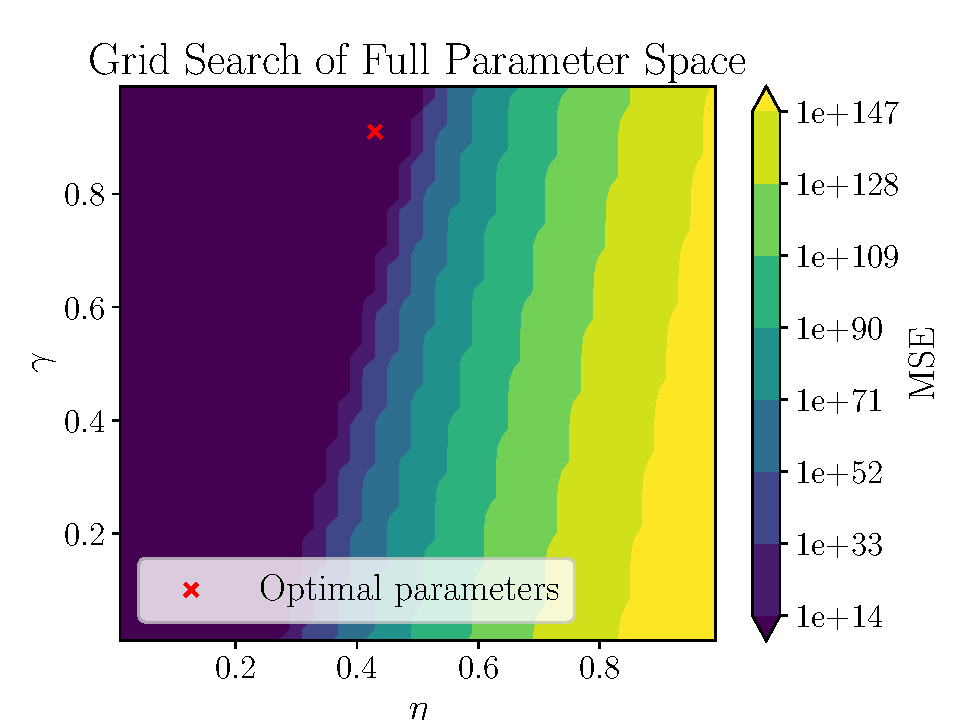
\includegraphics[width = .475\textwidth]{../figs/a_2_parameter_overview.pdf}
    \caption{Overview of the entire parameter space, plotting learning rate against momentum,  using plain gradient descent. The optimal parameters are marked with a red cross, to use as a starting point for further analysis.}
    \label{fig: param_overview}
\end{figure}
\begin{figure}[ht!]
    \centering
    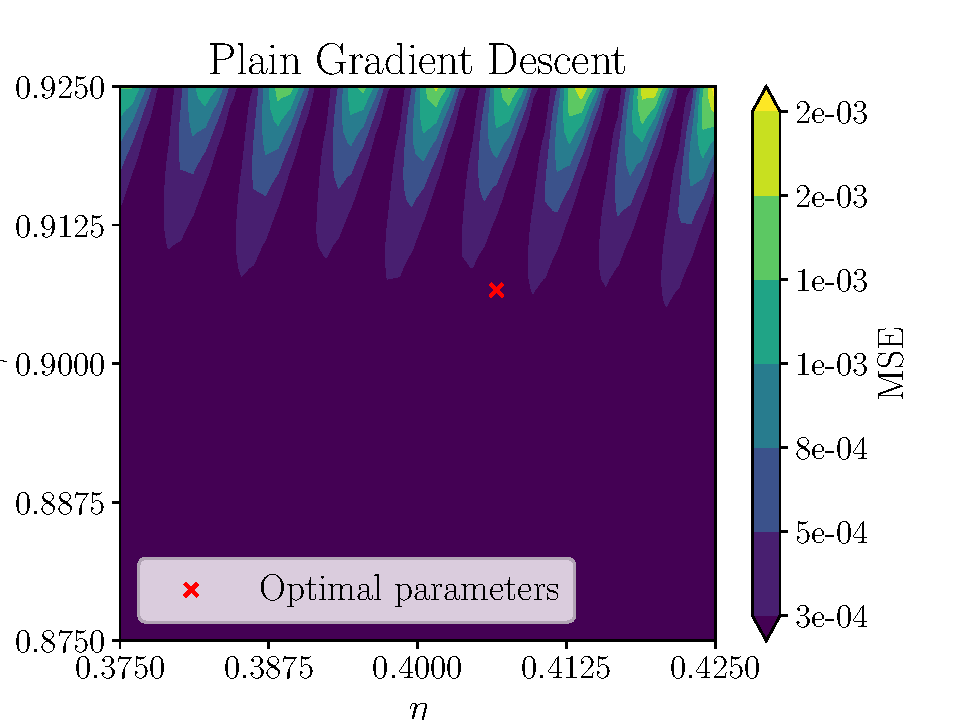
\includegraphics[width = .475\textwidth]{../figs/GD_eta_gamma.pdf}
    \caption{Narrowed down parameter space from \cref{fig: param_overview}.}
    \label{fig: param_narrowed}
\end{figure}
\begin{figure}[ht!]
    \centering
    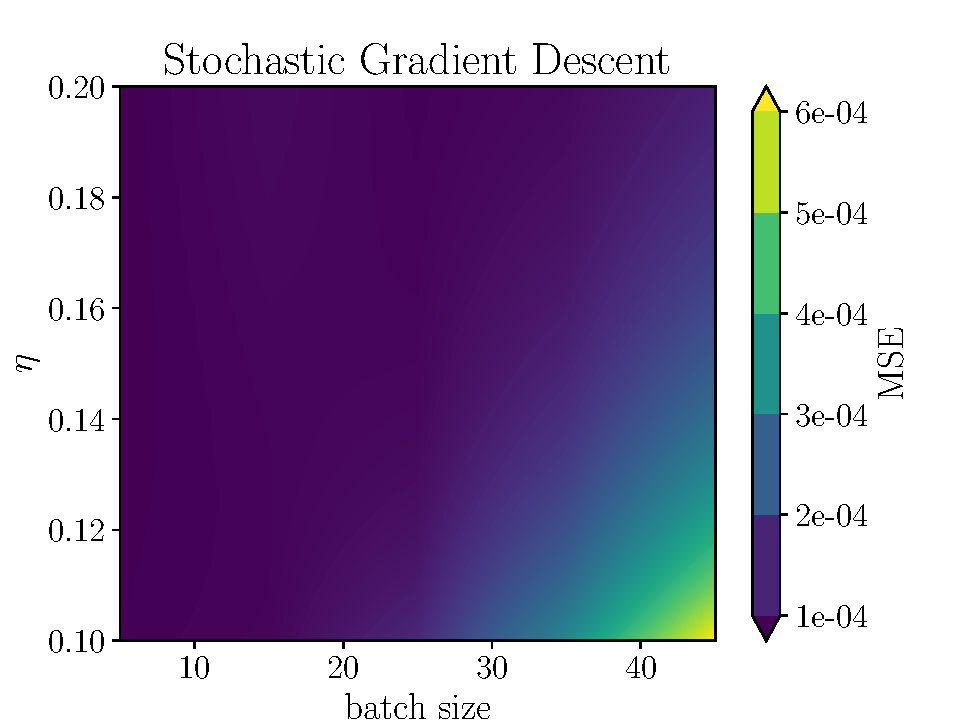
\includegraphics[width = .475\textwidth]{../figs/SGD_batch_eta_.pdf}
    \caption{Plotting batch size, against learning rate, using stochastic gradient descent.}
    \label{fig: SGD_batch_eta}
\end{figure}
\begin{figure}[ht!]
    \centering
    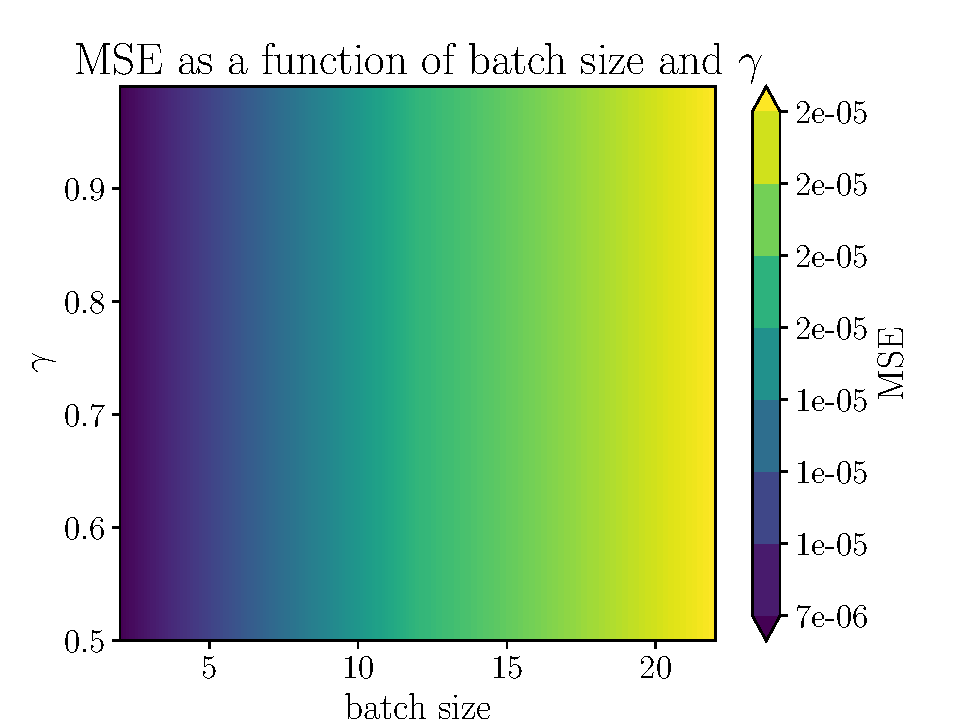
\includegraphics[width = 0.47575\textwidth]{../figs/SGD_batch_gamma.pdf}
    \caption{Plotting the batch size against the momentum, using stochastic gradient descent. Using a learning rate of $0.2$}
    \label{fig: SGD_batch_gamma}
\end{figure}

Looking at \cref{fig: param_overview} we found a region of parameters  in the upper-half , which gave the lowers MSE values. Using the best parameters found marked with a cross as a starting point, we found a good interval of values as seen in \cref{fig: param_narrowed}, with an order of magnitude around $10^{-4}$ and $10^{-3}$. In the following results, we only present the best intervals.

Continuing our search for the optimal batch number, we found between 5 and 20 batches to work well. In \cref{fig: SGD_batch_eta} without momentum. As a learning of $0.2$ gave the best results, we used this as our fixed learning rate in \cref{fig: SGD_batch_gamma} to find an optimal number of batches as a function of momentum. We see that the effect of changing the momentum is almost negligible, and that the number of batches is the most important parameter to tune. Even though we see a clear gradient in the plot, we find a large area with MSE values in the order of magnitude of \(10^{-5}\). The same is true in \cref{fig: SGD_batch_eta}, where over half of the learning rates between $0.1$ and $0.2$ give MSE values around \(10^{-4}\).

\subsubsection{AdaGrad}
\begin{figure}[ht!]
    \centering
    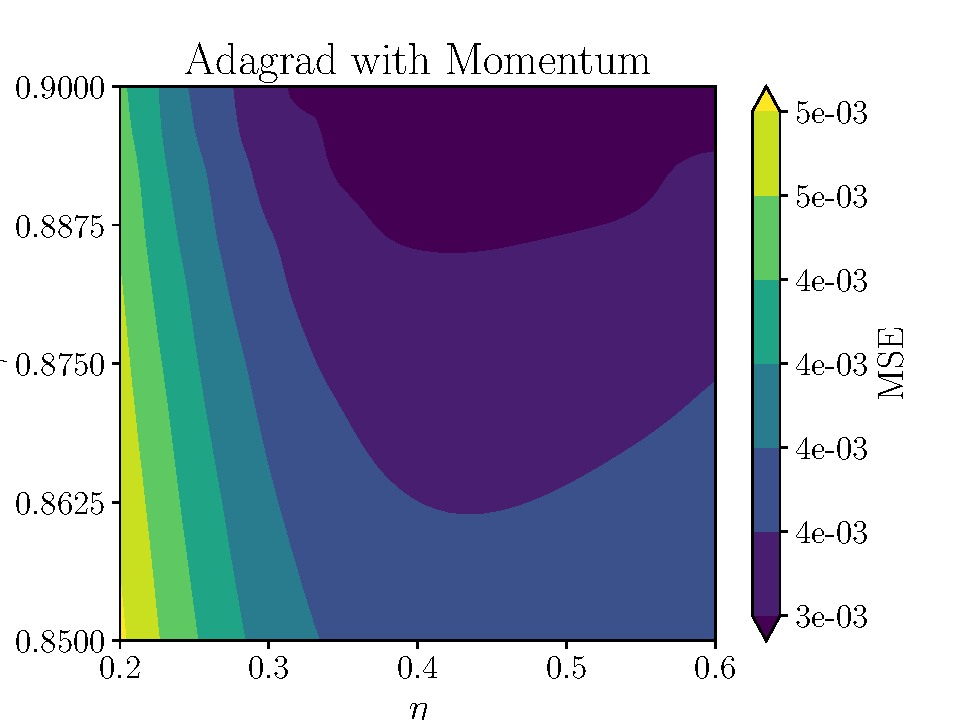
\includegraphics[width = 0.475\textwidth]{../figs/AdagradMomentum_eta_gamma.pdf}
    \caption{Plotting the learning rate against the momentum, using regular AdaGrad}
    \label{fig: AdagradMomentum_eta_gamma}
\end{figure}
\begin{figure}[ht!]
    \centering
    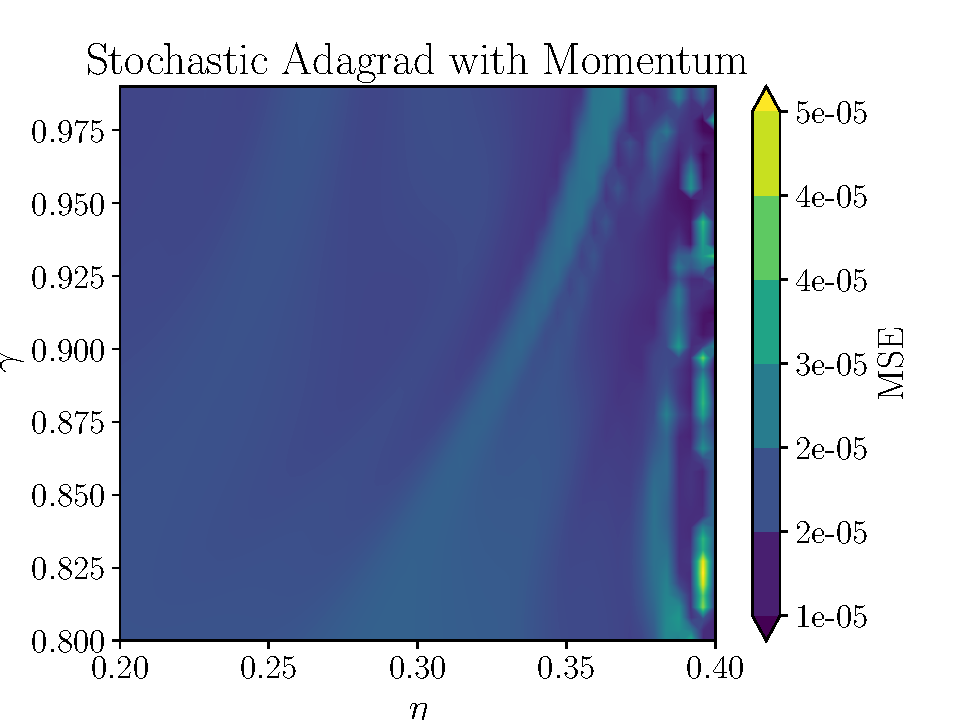
\includegraphics[width = 0.475\textwidth]{../figs/AdagradMomentum_stochastic_eta_gamma.pdf}
    \caption{Plotting the learning rate against the momentum, using stochastic AdaGrad. The batch size is set to 20.}
    \label{fig: AdagradMomentum_stochastic_eta_gamma}
\end{figure}
Exploring further with \cref{fig: AdagradMomentum_eta_gamma} and \cref{fig: AdagradMomentum_stochastic_eta_gamma} we found that the stochastic performed better then plain gradient descent, of 2 orders of magnitude. The stochastic version had an MSE of around \(10^{-5}\), while the plain version had an MSE of around \(10^{-3}\).

\subsubsection{RMSprop}
\begin{figure}[ht!]
    \centering
    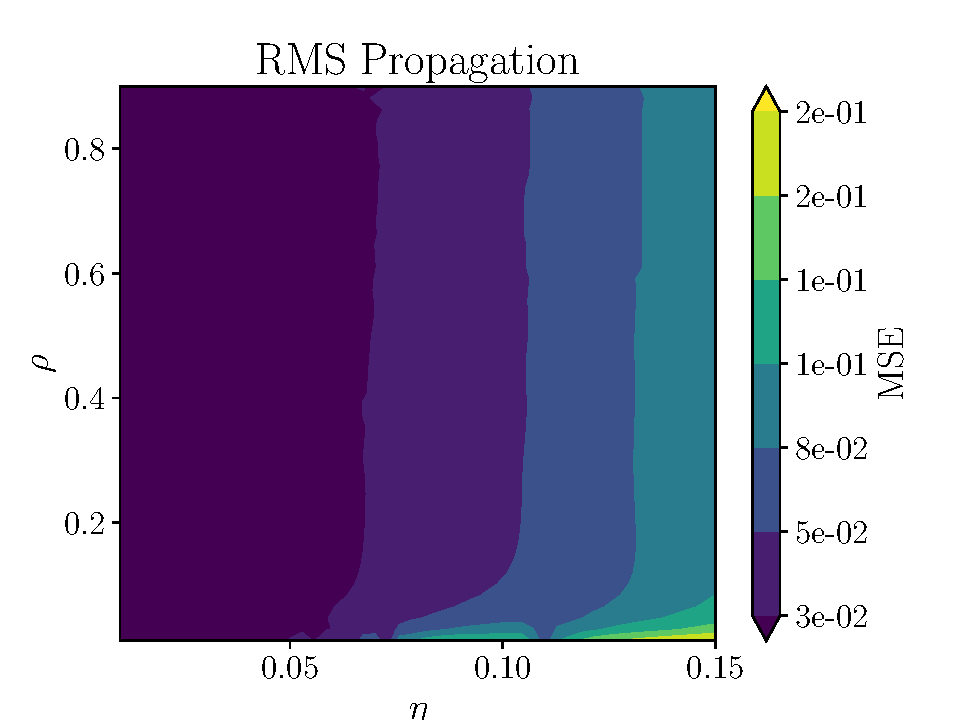
\includegraphics[width = 0.475\textwidth]{../figs/RMS_Prop_eta_rho.pdf}
    \caption{Plotting the learning rate against the decay rate, using RMSprop}
    \label{fig: RMS_Prop_eta_rho}
\end{figure}

\begin{figure}[ht!]
    \centering
    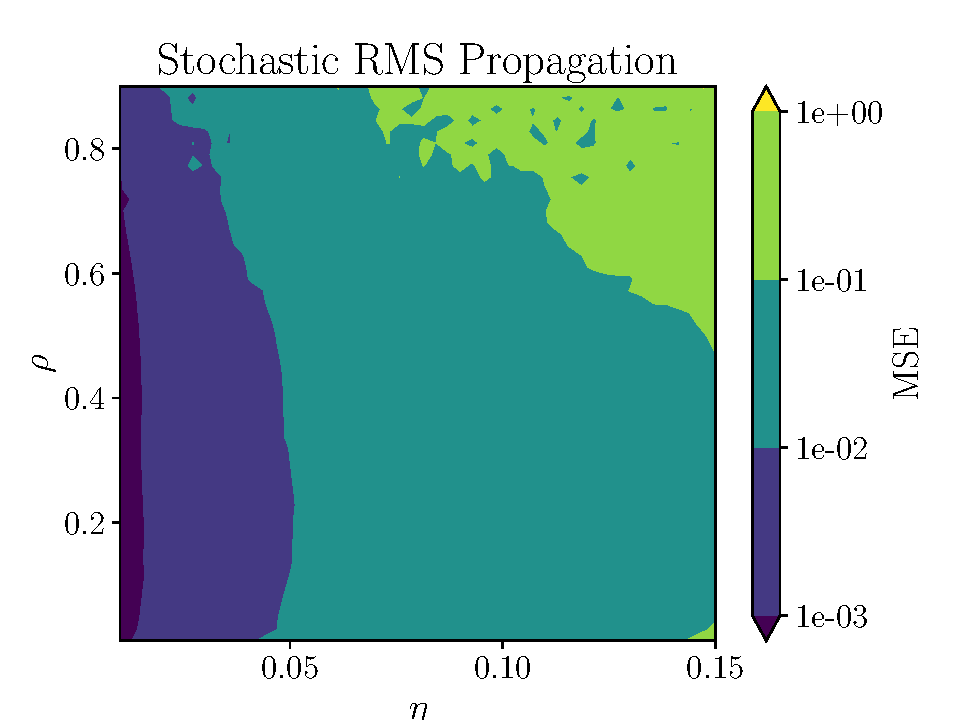
\includegraphics[width = 0.475\textwidth]{../figs/RMS_Prop_stochastic_eta_rho.pdf}
    \caption{Plotting the learning rate against the decay rate, using stochastic RMSprop. The batch size is set to 20.}
    \label{fig: RMS_Prop_stochastic_eta_rho}
\end{figure}
The RMS propagation method was very sensitive to the learning rate. As seen in \cref{fig: RMS_Prop_eta_rho} and \cref{fig: RMS_Prop_stochastic_eta_rho}, there was only a narrow range of learning rates that gave good results. Outside of this range, computation became unstable, and a lot of NaN values were produced. The stochastic version performed better than the plain version, with an MSE of around \(10^{-3}\) compared to \(10^{-2}\). Looking closer at the MSE values of the stochastic variant, we found some spots with MSEs with a value around \( 10^{-4} \). For the plain version, we found some spots with an MSE of around \( 10^{-3} \).

\subsubsection{Adam}
\begin{figure}[ht!]
    \centering
    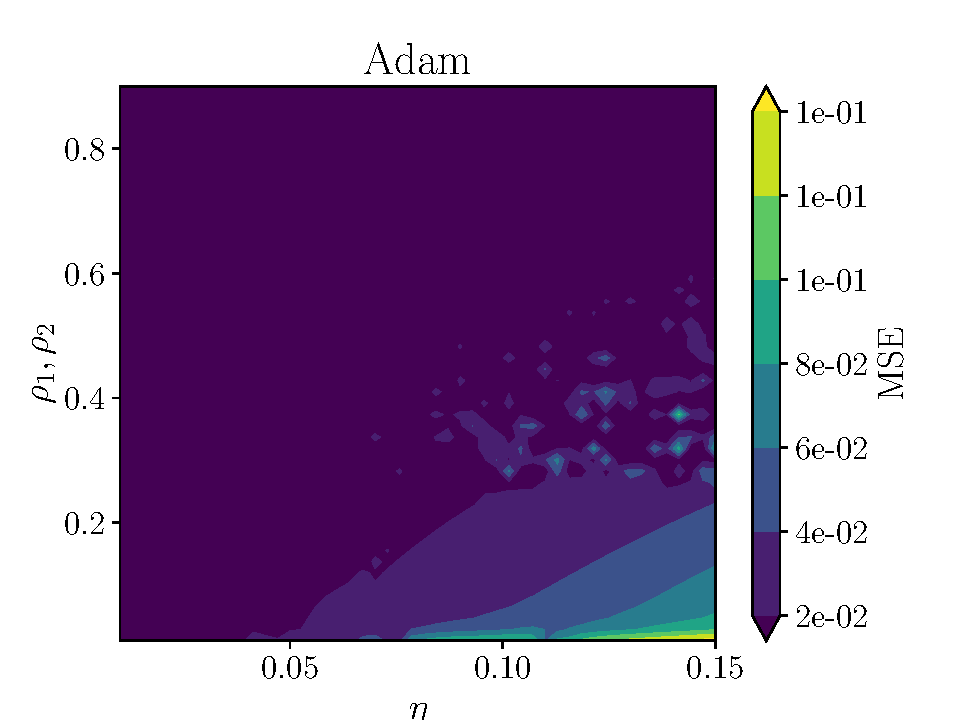
\includegraphics[width = 0.475\textwidth]{../figs/Adam_eta_rho.pdf}
    \caption{Plotting the learning rate against the decay rate. We have set the same value for $\rho_1$ and $\rho_2$, using Adam}
    \label{fig: Adam_eta_rho.pdf}
\end{figure}
\begin{figure}[ht!]
    \centering
    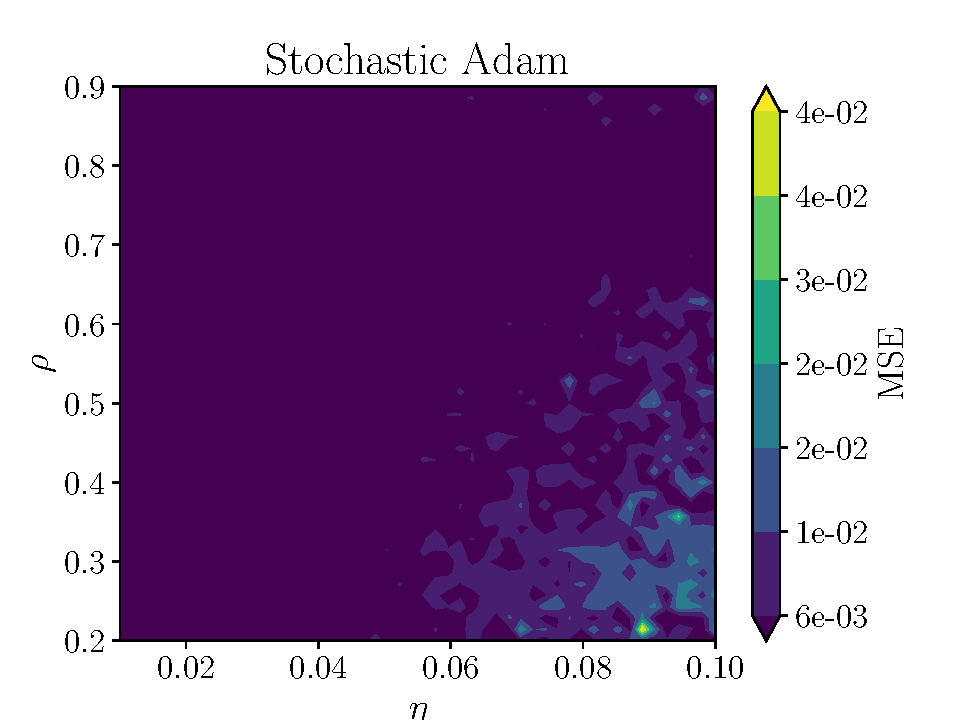
\includegraphics[width = 0.475\textwidth]{../figs/Adam_stochastic_eta_rho.pdf}
    \caption{Plotting the learning rate against the decay rate, using stochastic Adam. The batch size is set to 20, and the same value for $\rho_1$ and $\rho_2$ is used.}
    \label{fig: Adam_stochastic_eta_rho.pdf}
\end{figure}

The Adam optimization method was both unstable and very sensitive to the learning rate. As seen in \cref{fig: Adam_eta_rho.pdf} and \cref{fig: Adam_stochastic_eta_rho.pdf}, the plain version had at best an MSE of around \(10^{-2}\), while the stochastic version had an MSE of around \(10^{-3}\). The stochastic version had some spots with an MSE of around \(10^{-6}\). The plain version had some spots with an MSE of around \(10^{-4}\).

\subsection{Neural Networks Regression}

Our analysis of feed-forward neural networks began with the Franke function regression problem, allowing us to validate our implementation and explore the effects of various hyperparameters. The results demonstrate that our neural network implementation achieves robust performance across a wide range of configurations, with optimal models achieving MSE values around \( 10^{-3} \) and \( R^2 \) scores above 0.95.

\onecolumngrid
\begin{figure}[ht!]
    \centering
    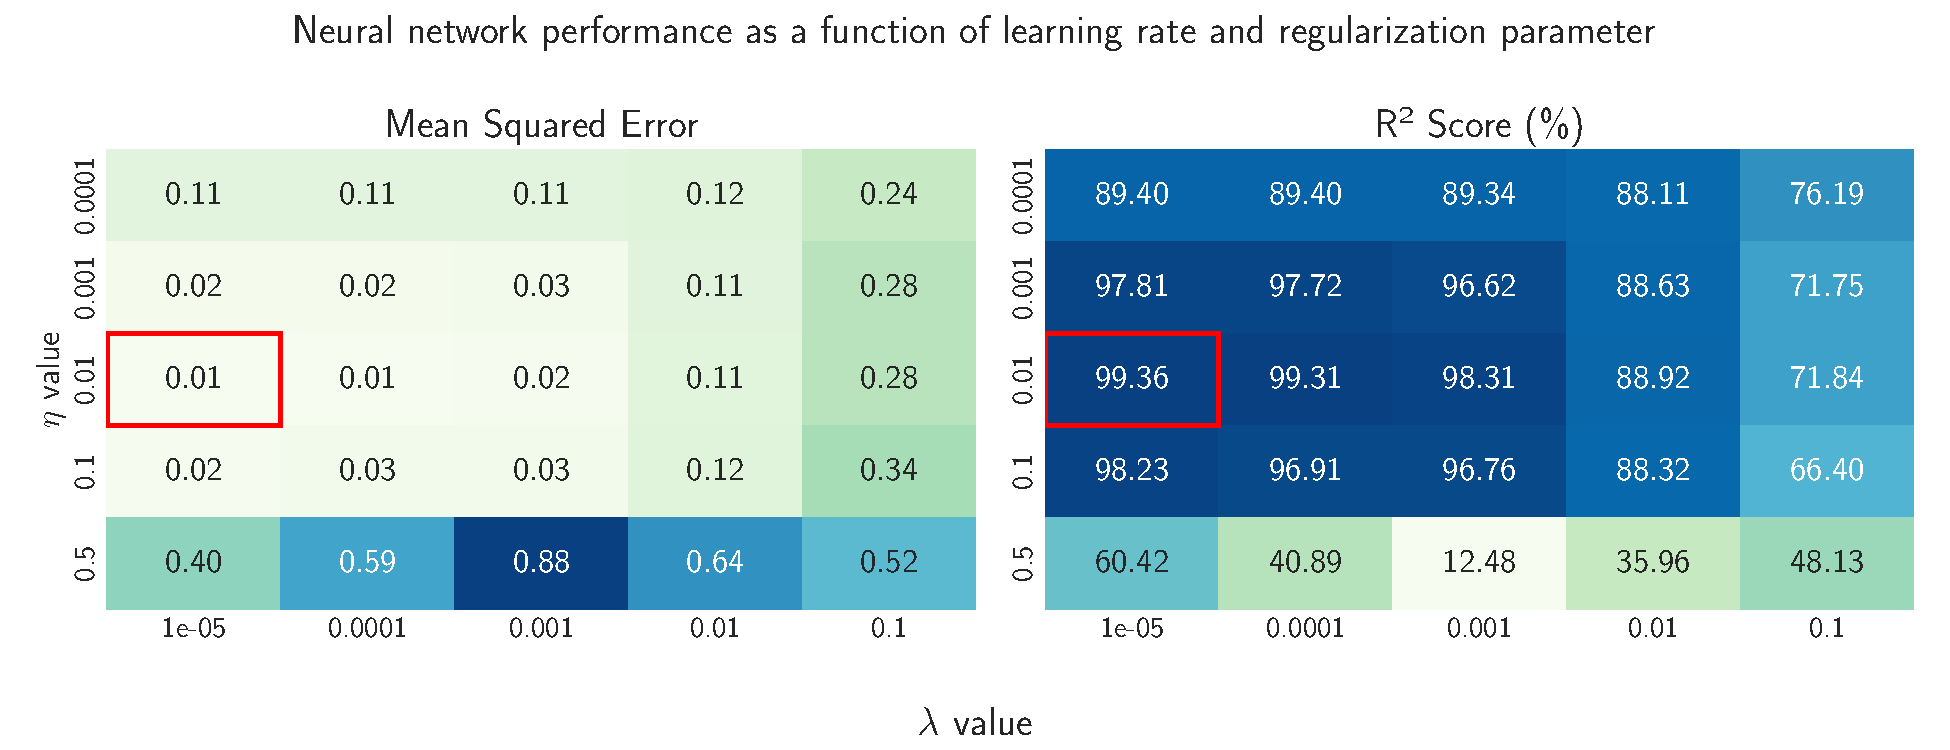
\includegraphics[width = .9\textwidth]{../figs/c_eta_lambda.pdf}
    \caption{The effect of learning rate and regularization strength on the Franke function regression problem. The plot shows the MSE and \( R^2 \) scores for different combinations of learning rate and regularization strength, with the optimal values highlighted in red.}
    \label{fig:NN_Franke_eta_lambda}
\end{figure}
\twocolumngrid

Our feed-forward neural network demonstrated consistently strong performance on the Franke function regression task across a range of hyperparameters. As shown in \cref{fig:NN_Franke_eta_lambda}, the model achieves stable MSE scores around $10^{-3}$ and $R^2$ scores above 0.99 for combinations of learning rates $ \eta $ in the range $ 10^{-1} $ to $ 10^{-3}$ and regularization strengths $ \lambda $ in $ 10^{-3} $ to $ 10^{-5}$ . The model only shows significant performance degradation with the highest tested learning rate ($\eta = 0.5$), suggesting robust behavior across most of the hyperparameter space.

\onecolumngrid
\begin{figure}[ht!]
    \centering
    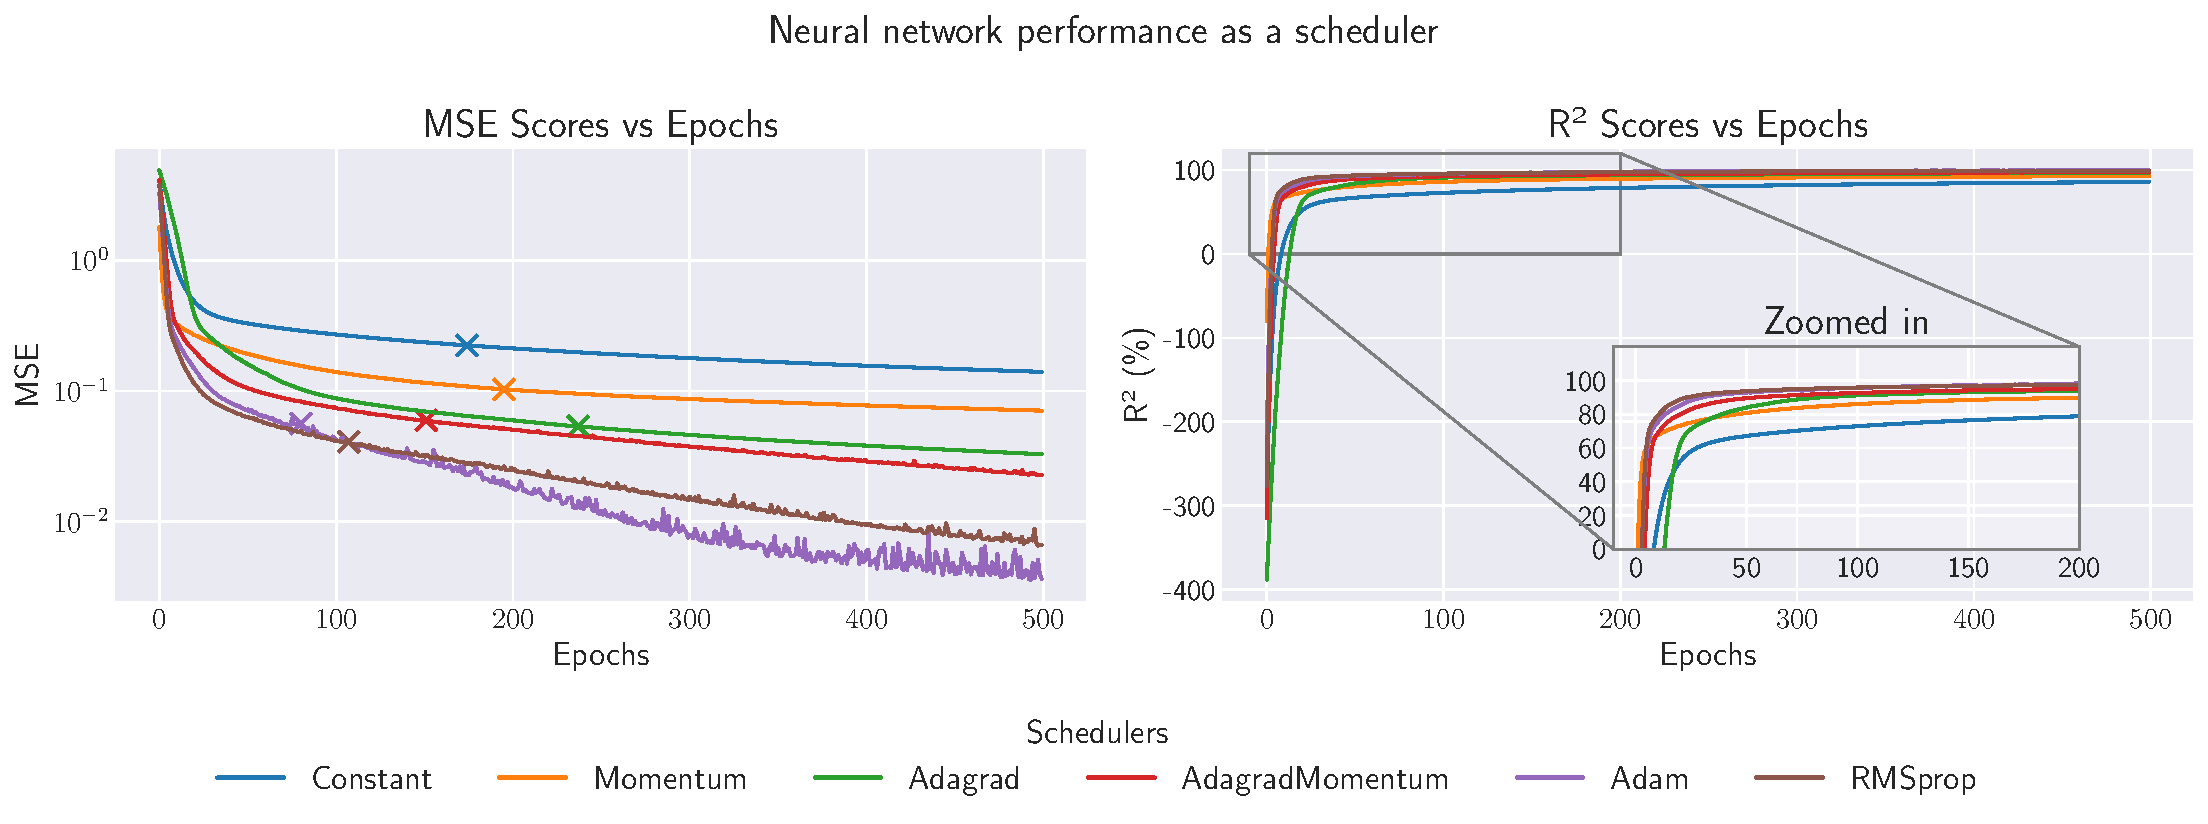
\includegraphics[width = .9\textwidth]{../figs/b_schedulers.pdf}
    \caption{The effect of different learning rate schedulers on the Franke function regression problem. The plot shows the training MSE and \( R^2 \) scores for different learning rate schedulers as a function of epochs. The schedulers MSEs are marked with a cross indicating at which epoch convergence was reached.}
    \label{fig:NN_Franke_schedulers}
\end{figure}
\twocolumngrid

The comparison of different optimization schedulers in \cref{fig:NN_Franke_schedulers} shows that all implemented methods have varying success with Adam and RMSprop performing the best. The marked convergence points indicate that both Adagrad methods are slower to converge than the other methods, while RMSprop reach its point around just 100 epochs. As the criteria for convergence is chosen somewhat arbitrarily, as describe in \cref{subsec:nn_schedulers}, the marked crosses may not showcase where the schedulers converge, but gives insight into when the learning rates are slowing down relative to eachother as the networks are training. The figure also suggest that given enough epochs, both Adagrads, Adam and RMSprop will converge to an mse of just short of \( 10^{-3} \) and an \( R^2 \) score of 0.95. While constant learning rate and plain momentum will perform worse.

\onecolumngrid
\begin{figure}[ht!]
    \centering
    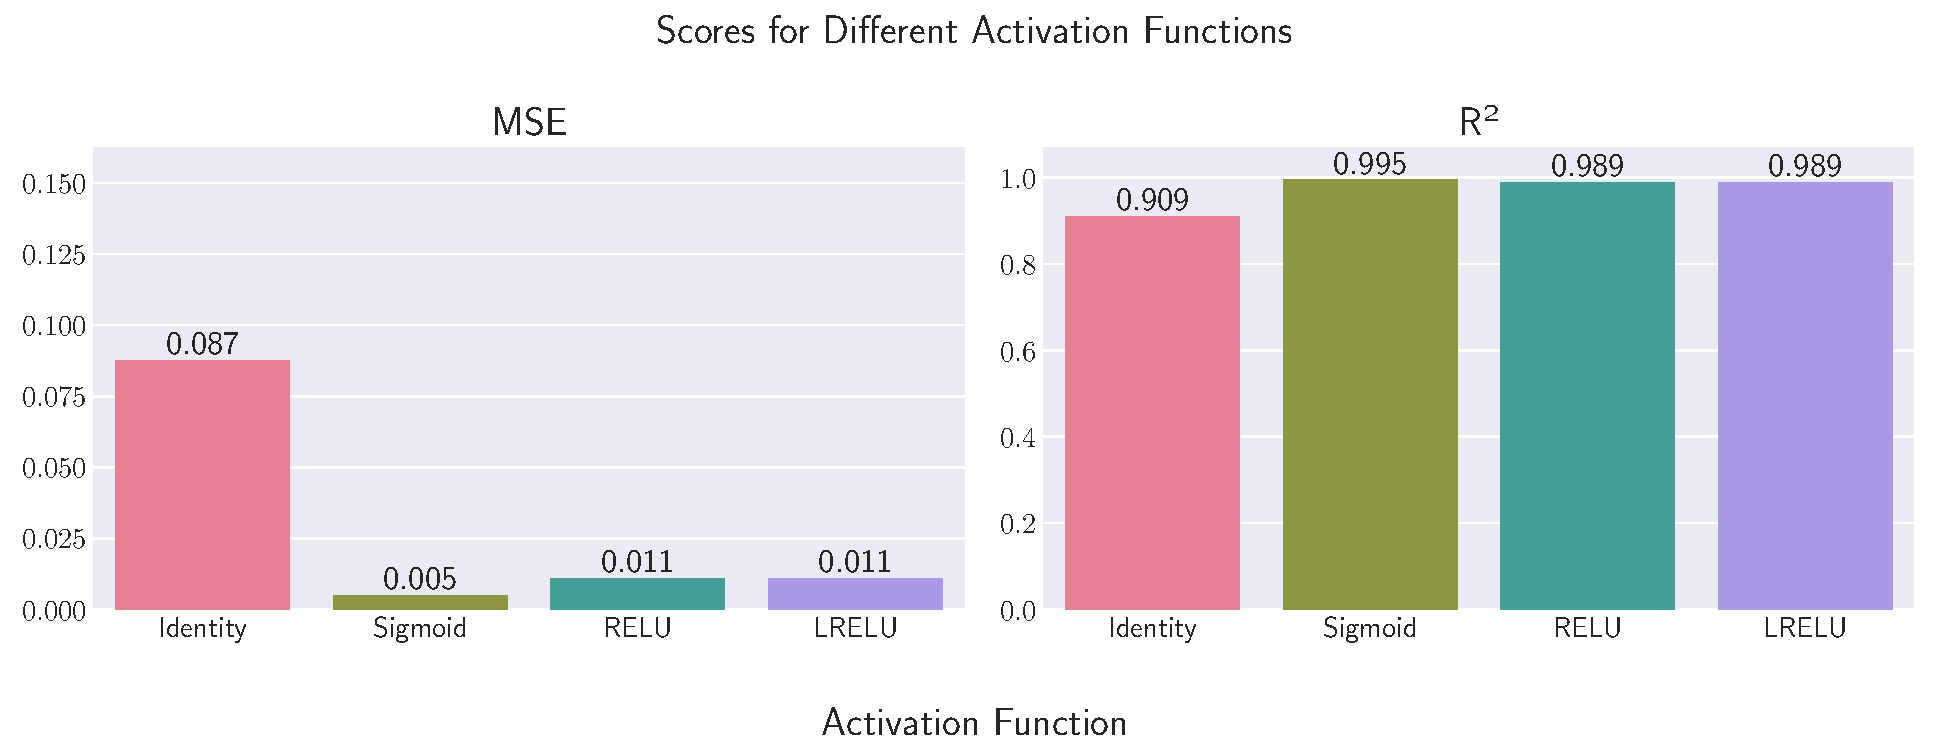
\includegraphics[width = .9\textwidth]{../figs/c_activation_funcs.pdf}
    \caption{The effect of different activation functions on the Franke function regression problem. The plot shows the test MSE and \( R^2 \) scores for different activation functions.}
    \label{fig:NN_Franke_activation}
\end{figure}
\twocolumngrid

Testing different activation functions (\cref{fig:NN_Franke_activation}), reveals similar performance levels among non-linear functions. The sigmoid activation in the hidden layer performs slightly better with an MSE of $0.005$ and $R^2$ of $0.995$, but ReLU and Leaky ReLU follow closely with MSE around $0.011$ and $R^2$ of $0.989$. As expected, removing the non-linear capability of the network by using the identity function in the hidden layer results in significantly worse performance, with an MSE of $\approx 0.09$ and $R^2$ of $\approx0.91$.

\onecolumngrid
\begin{figure}[ht!]
    \centering
    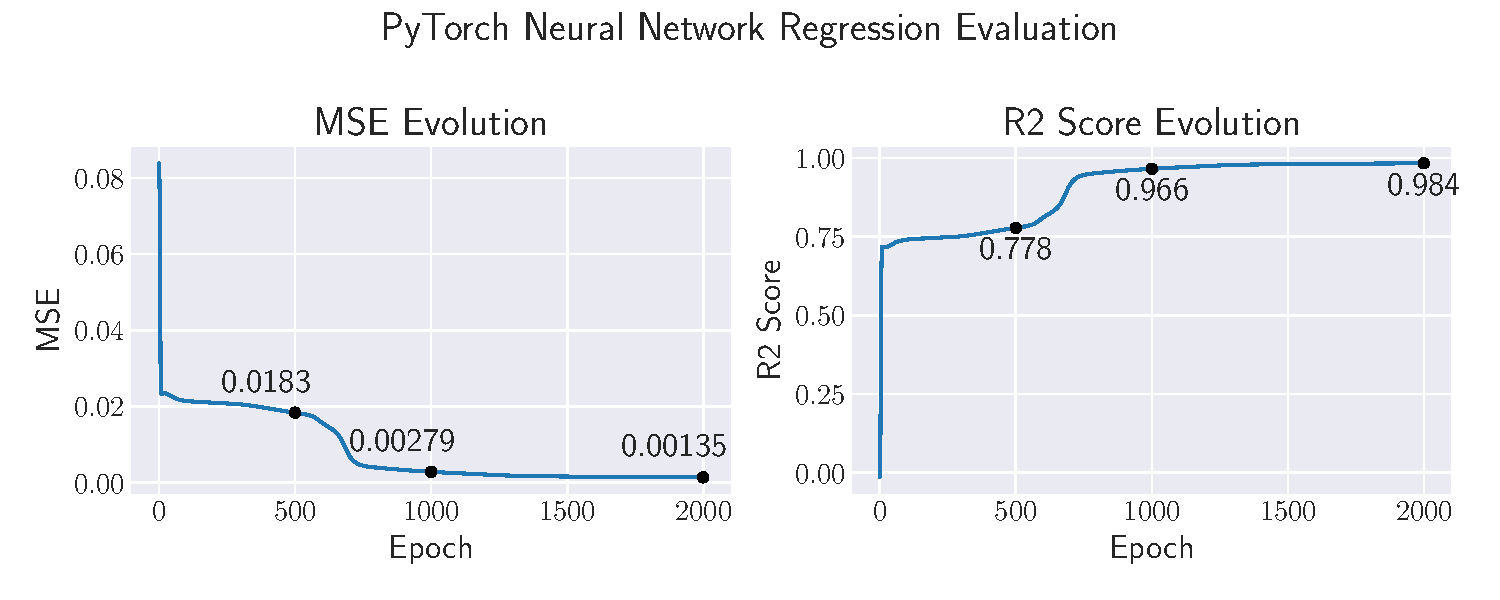
\includegraphics[width = .9\textwidth]{../figs/nn_torch_franke.pdf}
    \caption{PyTorch neural network regression on the Franke function. The plot shows the training and test MSE and \( R^2 \) as a function of epochs. The plots are annotated with the values at epochs 500, 1000 and 2000}
    \label{fig:NN_Torch_scores}
\end{figure}
\twocolumngrid

Comparing our results with the PyTorch implementation in \cref{fig:NN_Torch_scores}, we see that our model performed similarly to the PyTorch model, with an MSE around \( 10^{-3} \) and an \( R^2 \) score around 0.95. The main takeaway from this is that our models were faster to reach stable performance, wile the PyTorch model took more epochs to become stable at slightly better performance. This might suggest that the PyTorch model is more robust to overfitting, but at the cost of longer training times.

\clearpage

\subsection{Neural Networks Classification}

\onecolumngrid
\begin{figure}[ht!]
    \centering
    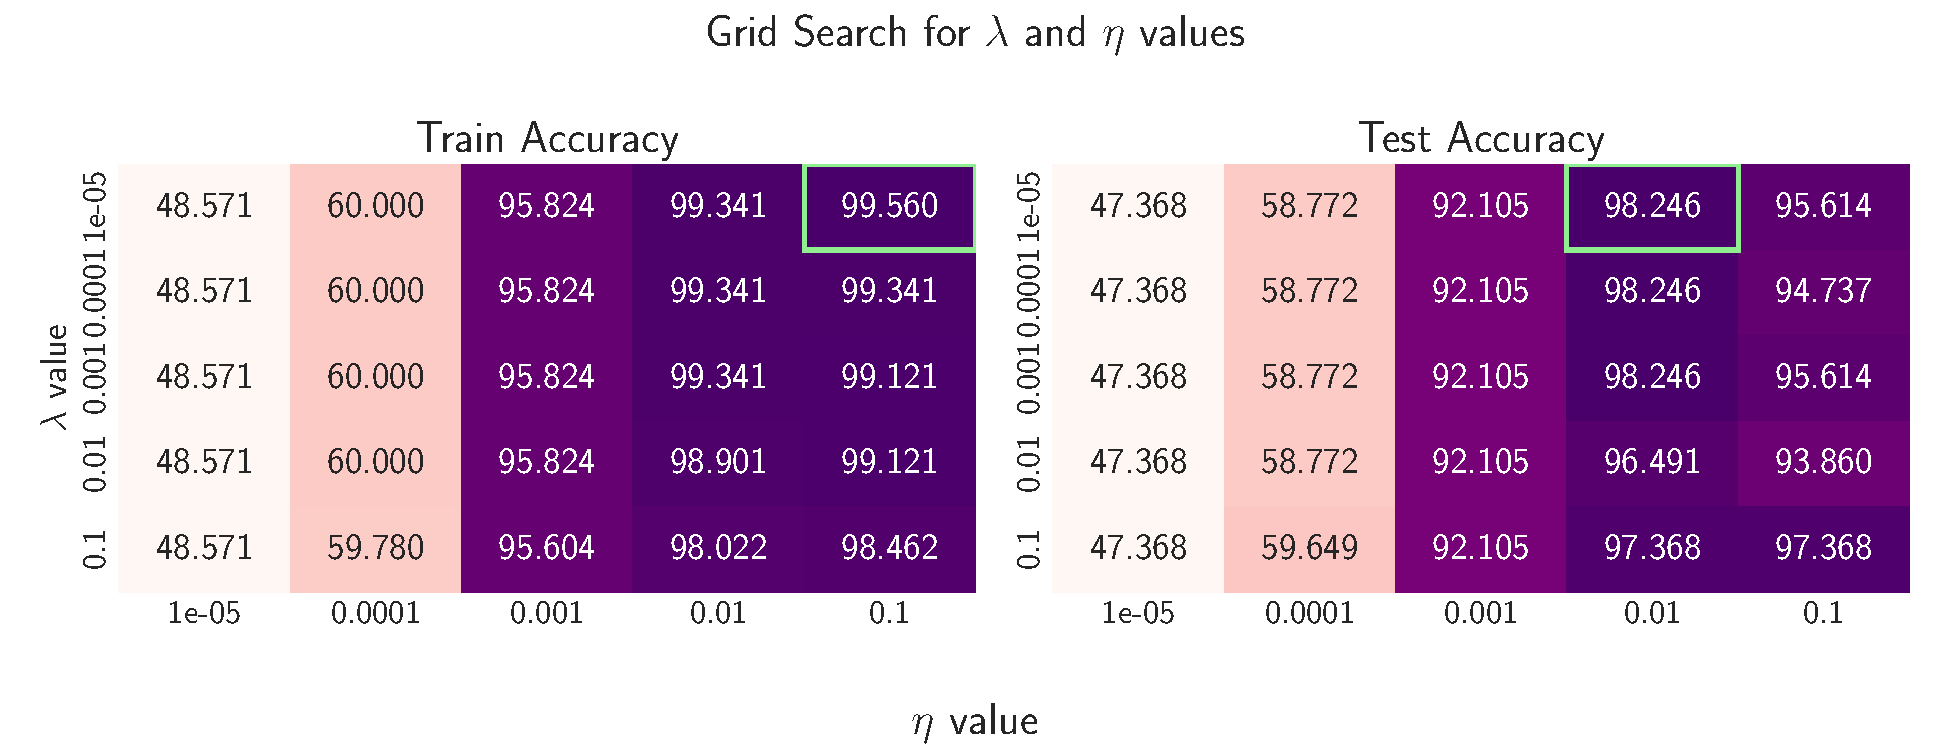
\includegraphics[width = .9\textwidth]{../figs/classification_lambda_eta.pdf}
    \caption{Model performance for different learning rates and regularization strengths on the breast cancer classification problem. The plot shows the training and test accuracy scores for different combinations of learning rate and regularization strength. The optimal values are highlighted in green.}
    \label{fig:NN_Classification_lambda_eta}
\end{figure}
\twocolumngrid

Our feed-forward neural network achieved strong classification performance on the Wisconsin Breast Cancer dataset. As shown in \cref{fig:NN_Classification_lambda_eta}, the model maintains high accuracy ($<95\%$) across a broad range of hyperparameter combinations. Performance is most dependent on the learning rate, having optimal performance for $\eta$ between $10^{-1}$ and $10^{-2}$, while the regularization strength is less critical with a slight trend for better performance with lower $\lambda$ values. In the figure, the optimal values for training accuracy and test accuracy differ. Since the dataset is small, the model is prone to overfitting and this could be the reason for the discrepancy.

\onecolumngrid
\begin{figure}[ht!]
    \centering
    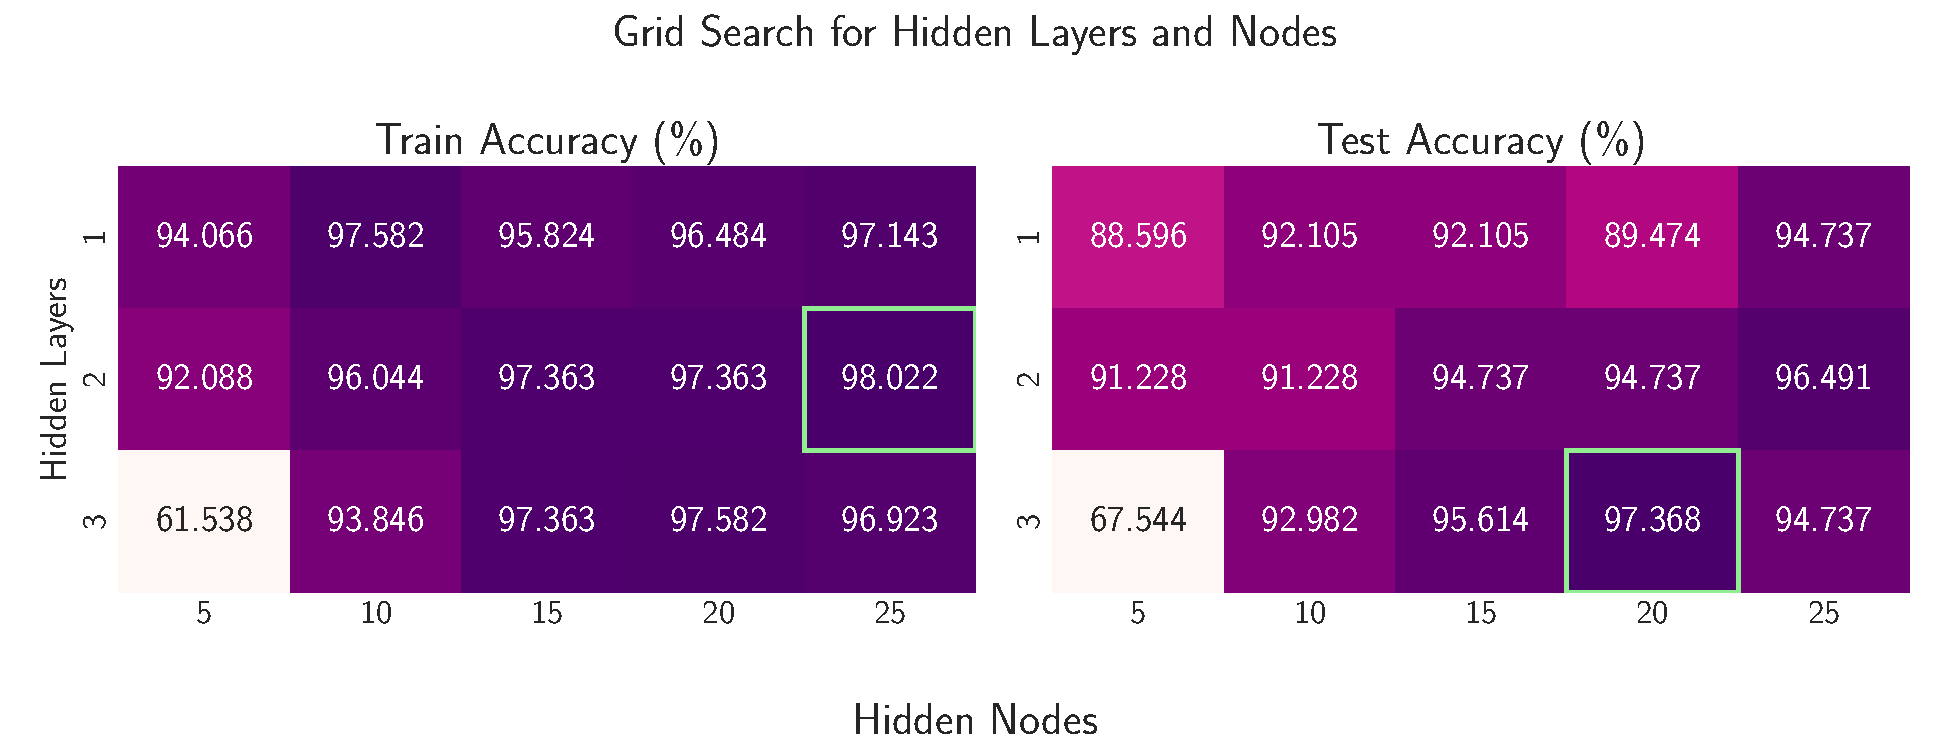
\includegraphics[width = .9\textwidth]{../figs/classification_hidden_layers_nodes.pdf}
    \caption{Model performance for different network architectures on the breast cancer classification problem. The plot shows the training and test accuracy scores for different numbers of hidden layers and nodes. The optimal values are highlighted in green.}
    \label{fig:NN_Classification_hidden_layers_nodes}
\end{figure}
\twocolumngrid

The exploration of network architectures demonstrates that model performance remains robust across different configurations. Networks with 2-3 hidden layers and 15-25 nodes per layer consistently achieve test accuracies above 96\%. Notably, very small networks (5 nodes) show degraded performance, particularly with three layers where training accuracy drops to 61.5\%, suggesting insufficient model capacity. Our initial assumptions that it would suffice to have a small network for this dataset are somewhat backed up by the results, but the faster runtimes do have a tradeoff in performance.

\onecolumngrid
\begin{figure}[ht!]
    \centering
    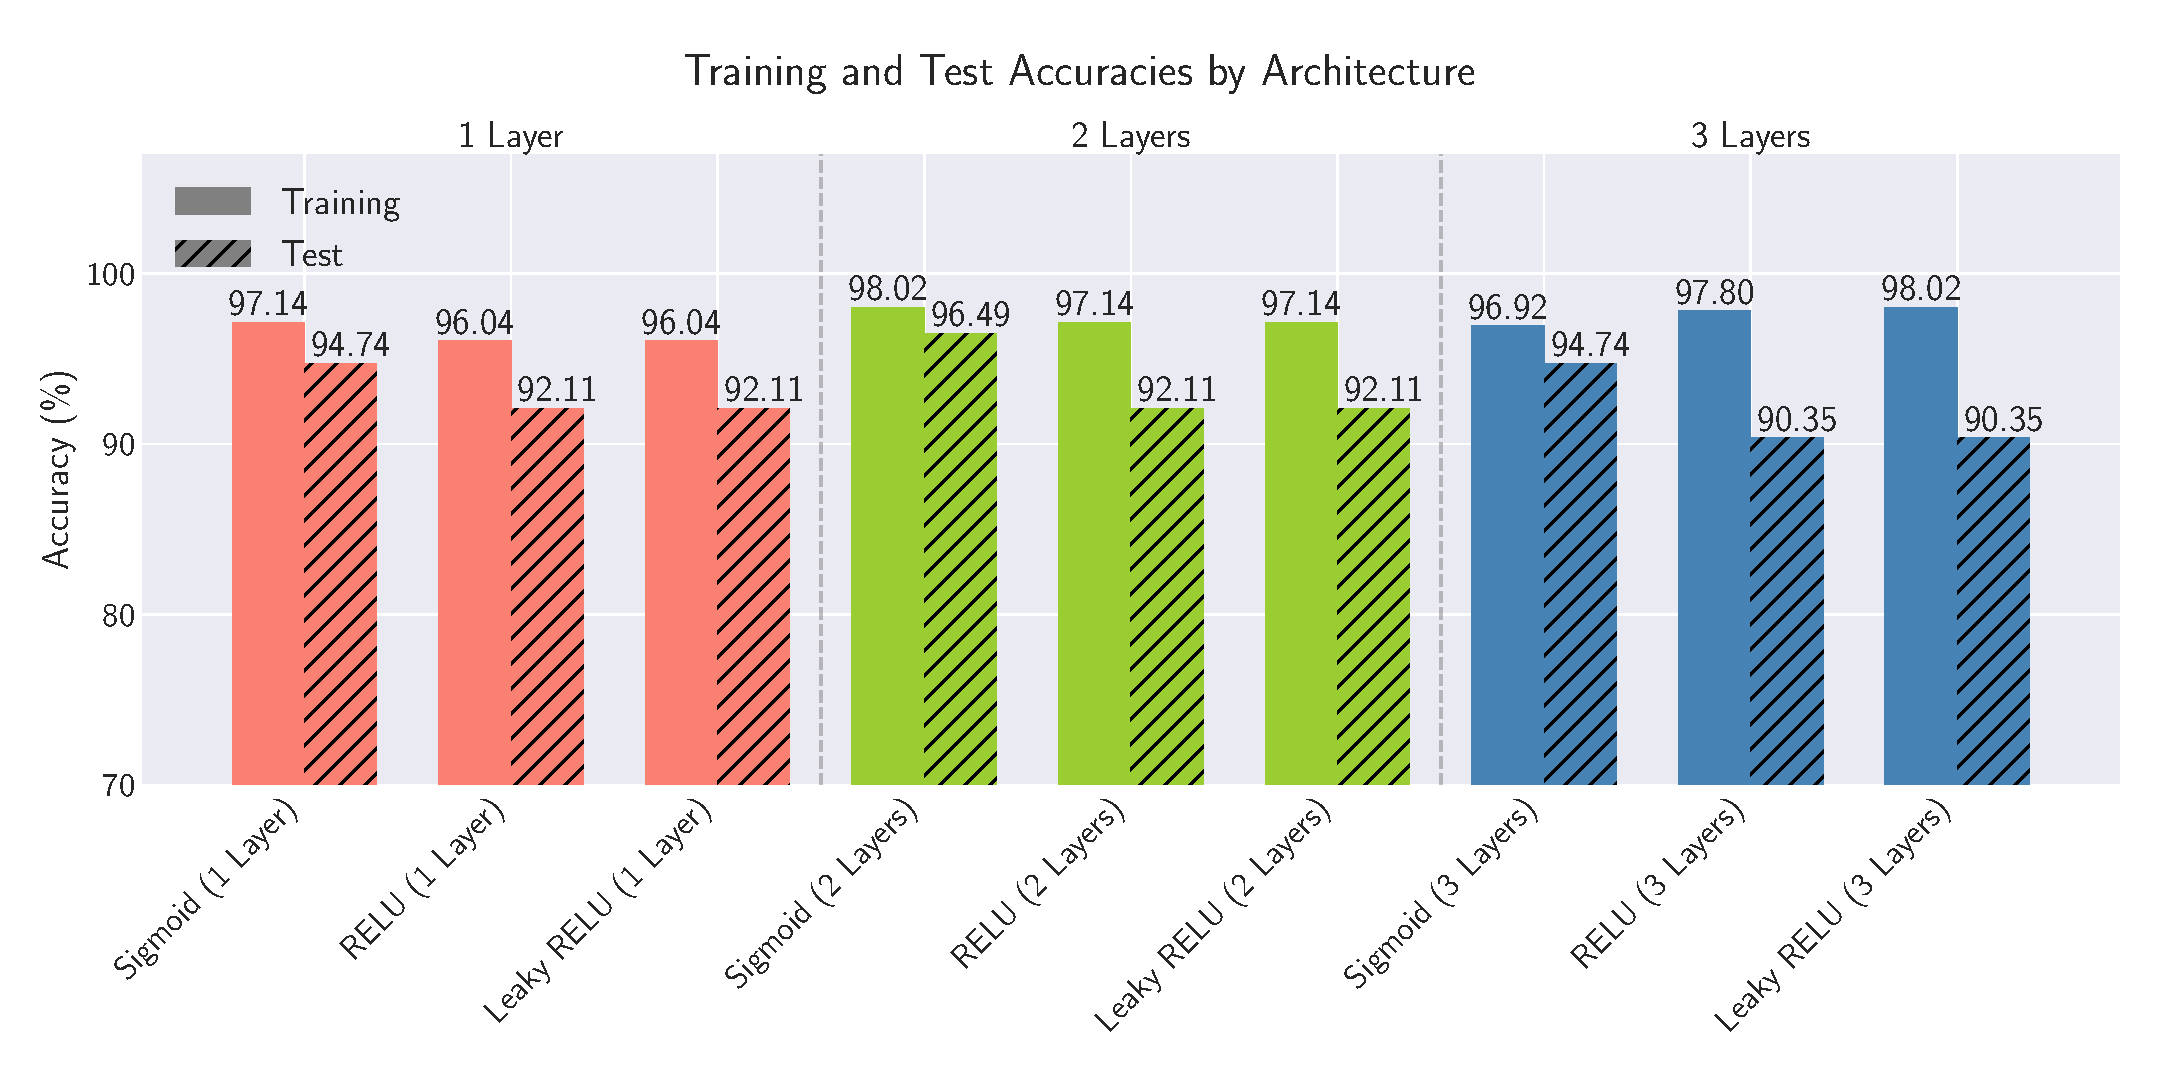
\includegraphics[width = .9\textwidth]{../figs/classification_activations_layers.pdf}
    \caption{Model performance for different activation functions on the breast cancer classification problem. The plot shows the training and test accuracy scores for different activation functions and numbers of hidden layers.}
    \label{fig:NN_Classification_activations_layers}
\end{figure}
\twocolumngrid

All tested activation functions perform similarly well, with accuracy variations within 2-3 percentage points. In single-layer configurations, sigmoid achieves slightly better performance, while ReLU and Leaky ReLU trends to better performance in deeper networks. This is only true for the training data, as all test accuracies degrade with more layers. This again suggest the danger of overfitting, and that the dataset is too small to support deep networks.

\begin{figure}[ht!]
    \centering
    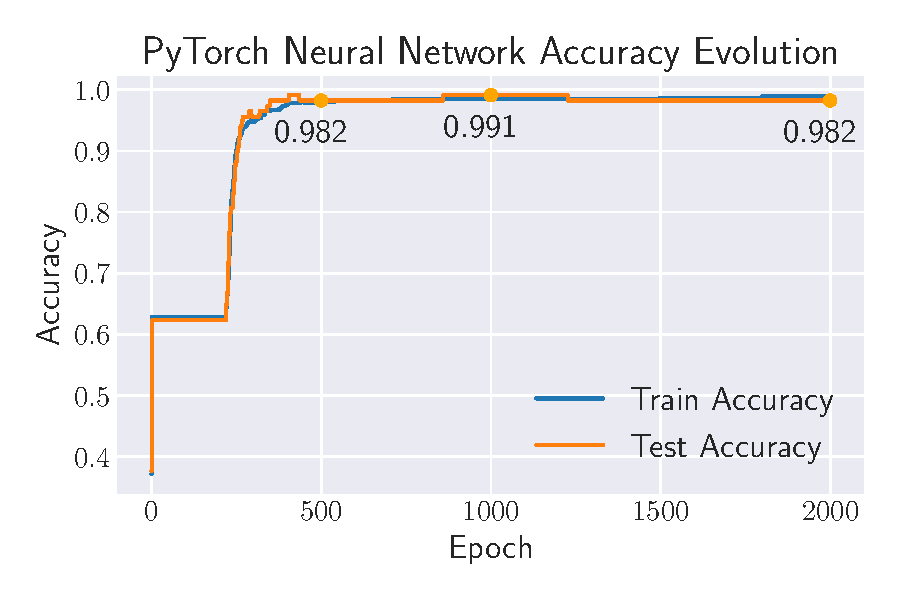
\includegraphics[width =.45\textwidth]{../figs/nn_torch_breast_cancer.pdf}
    \caption{PyTorch neural network classification on the breast cancer dataset. The plot shows the training and test accuracy as a function of epochs. The figure is annotated with the test accuracies at epochs 500, 1000 and 2000.}
    \label{fig:NN_Torch_breast_cancer}
\end{figure}

From \cref{fig:NN_Torch_breast_cancer}, we see that the PyTorch model is a more stable model, taking more time to reach high performance levels, but manages to hold a test accuracy of $<98\%$ after 500 epochs. As our models are often scoring above 98\% after only 20 epochs. A possible explanation for this is that the PyTorch model is a more advanced model, increasing the difficulty to train the network compared to our relatively simple model for a small data set as the Wisconsin Breast Cancer data.

\subsection{Logistic Regression}

\onecolumngrid
\begin{figure}[ht!]
    \centering
    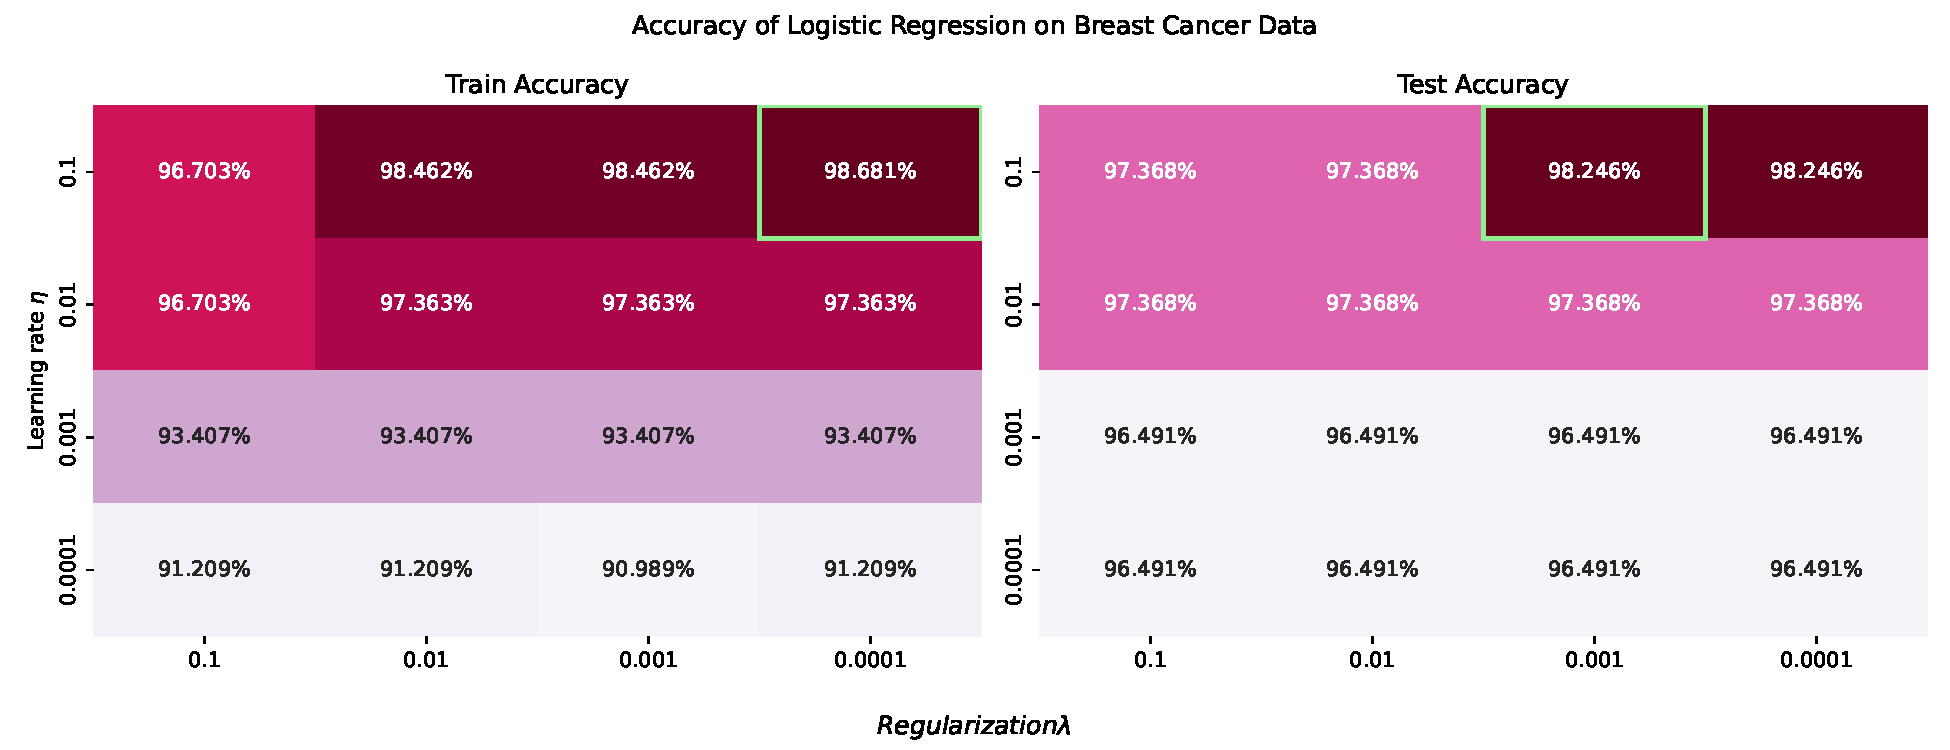
\includegraphics[width = .9\textwidth]{../figs/logistic_regression_gridsearch.pdf}
    \caption{Model performance for different learning rates and regularization strengths on the breast cancer classification problem using logistic regression. The plot shows the training and test accuracy scores for different combinations of learning rate and regularization strength. The optimal values are highlighted in green.}
    \label{fig:logistic_regression_gridsearch}
\end{figure}
\twocolumngrid

Our logistic regression implementation achieves high performance on the breast cancer dataset, with test accuracies consistently above 96\% across most hyperparameter combinations. \cref{fig:logistic_regression_gridsearch} shows that performance is robust across a wide range of learning rates and regularization strengths, with optimal test accuracy of 98.2\% achieved at $\eta$ = 0.0001 and a regularization strength of 0.1. The model demonstrates good generalization, with test accuracies closely matching training accuracies across the parameter space.

\begin{figure}[ht!]
    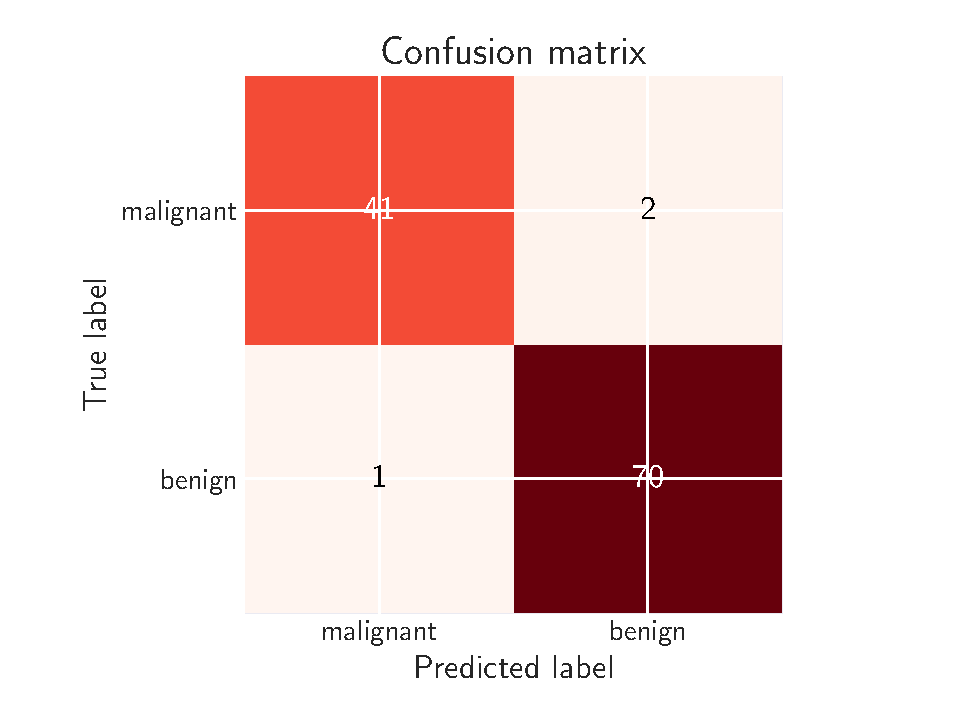
\includegraphics[width =.45\textwidth]{../figs/confusion_matrix.pdf}
    \caption{Confusion matrix for the breast cancer classification problem with Skikit's Logistic Regression. The plot shows the confusion matrix for the test set, with the number of true positives, true negatives, false positives, and false negatives.}
    \label{fig:confusion_matrix}
\end{figure}

The confusion matrix from scikit-learn's implementation (\cref{fig:confusion_matrix}) shows excellent classification performance with only 3 misclassified samples out of 114 test cases. The model correctly identified 41 out of 43 malignant cases and 70 out of 71 benign cases, demonstrating balanced performance across both classes. The similar performance between our implementation and scikit-learn's validates our approach while suggesting that the classification task may be well-suited for linear decision boundaries.

\clearpage

% \vspace*{-2.5pt}


\section{Conclusion}\label{sec:conclusion}
% \vspace*{-2.5pt}
In this study, we have implemented and analyzed various optimization algorithms and neural network architectures for bot regression and classification tasks. Our regression analysis demonstrated mixed success across different optimization method. While plain gradient descent and stochastic gradient descent with AdagGrad achieved satisfactory result performance with MSE values around $ 10^{-5} $, we encountered challenges in optimizing the hyperparameter for RMSprop and Adam. These methods showed inconsistent performance, with occasional regions of good convergence (MSE $\approx 10^{-5}$) amid generally poorer results (MSE $\approx 10^{-1}$). 

The neural network implementation proved more robust, particularly in regression task using the Franke function. Our systematic analysis of hyperparameter revealed optimal configurations achieving MSE values of $10^{-3}$ and $R^2$ scores above 0.99. The comparison of different activation functions showed that while sigmoid activation performed marginally better (MSE $\approx 0.003$), both ReLU and Leaky ReLU maintained strong performance (MSE $\approx 0.010$), demonstrating the flexibility of our implementation.

For the classification task using the Wisconsin Breast Cancer dataset, our neural network achieved impressive accuracy ($>98\%$) across various architectures, notably performing on par with and occasionally exceeding the PyTorch implementation. However, this result should be interpreted with caution given the relatively small dataset size. The observed rapid convergence of our model, while computationally efficient, may indicate premature settling into local minima rather than finding truly optimal solutions.

Several areas warrant further investigation, particularly given the constraints of our current study. Due to computational limitations, we significantly restricted our hyperparameter search space, exploring only a modest range of learning rates, batch sizes, and network architectures. The runtime constraints also limited our ability to test higher polynomial degrees and more complex network configurations, especially for the regression task. A more comprehensive study with access to greater computational resources could explore:

\begin{itemize}
    \item Broader hyperparameter spaces, particularly for RMSprop and Adam optimization
    \item Larger network architectures with more hidden layers and nodes
    \item Higher polynomial degrees for the regression analysis
    \item More extensive cross-validation and ensemble methods
    \item The effect of different initialization strategies
    \item Alternative regularization techniques beyond L2 regularization
\end{itemize}

Additionally, while our neural network performed well on both tasks, a more extensive analysis of its behavior on larger datasets would better validate its generalization capabilities. The relationship between network depth and overfitting, particularly evident in the classification task, merits deeper exploration to establish more reliable guidelines for architecture selection.
% \section*{Acknowledgements}\label{sec:cknowledgements}
% % MAYBE REMOVE

\Urlmuskip=0mu plus 1mu\relax
\onecolumngrid
\bibliography{references}

\newpage
% ===========================================
\appendix
\section{Code}\label{appsec:code}
Link to our GitHub repository: \href{https://github.com/Oskar-Idland/FYS-STK4155-Projects}{https://github.com/Oskar-Idland/FYS-STK4155-Projects}

\section{Additional Figures}\label{appsec:figures}
\begin{figure}[h!]
    \centering
    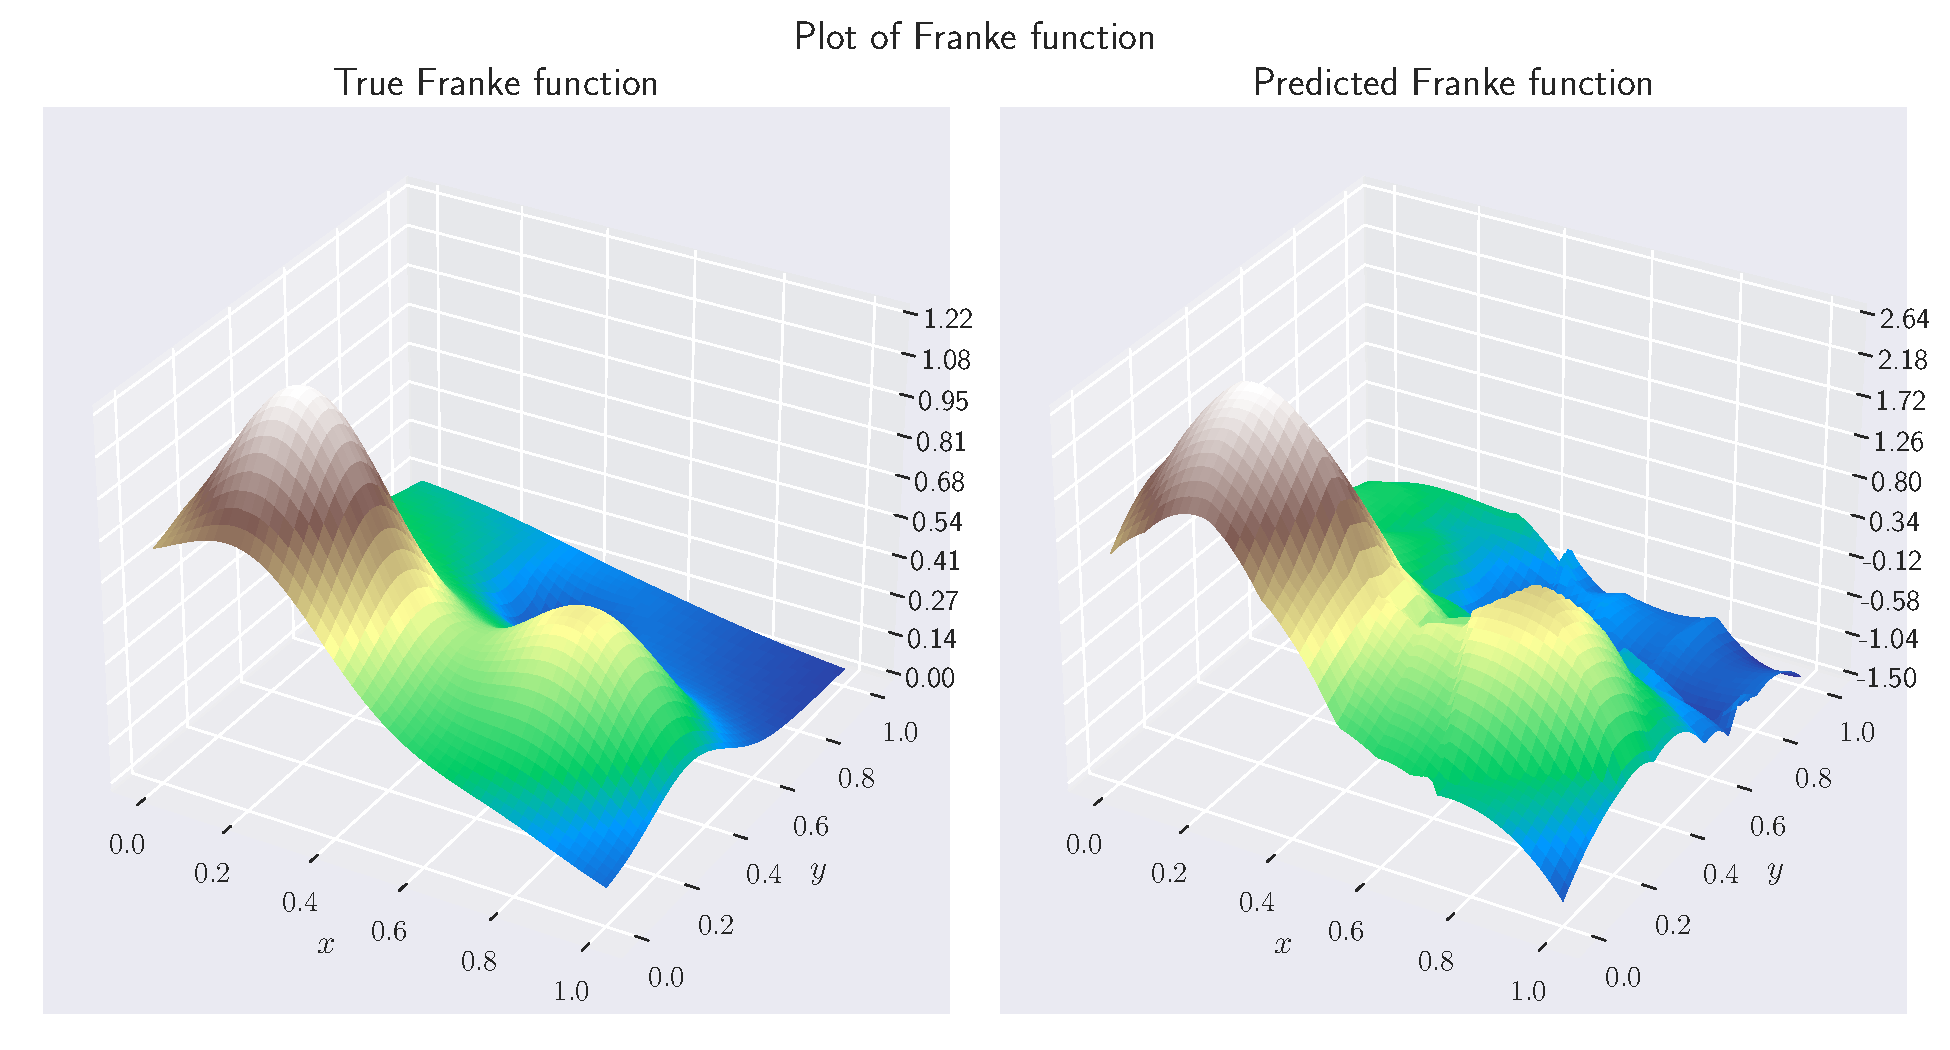
\includegraphics[width=0.9\columnwidth]{../figs/franke_model_pred.pdf}
    \caption{Plotted prediction of the Franke function using an optimal model that strikes balance between performance and computational efficiency. The model is a neural network with a single hidden layer of 15 neurons, trained with the Adam optimizer ($\eta = 0.001, \ \rho_1 = 0.9, \ \rho_2 = 0.999$)and Leaky ReLU activation function. The model was trained for 1000 epochs with 20 batches and a regularization strength of $\lambda = 0.0001$.}
    \label{fig:franke_model_pred}
\end{figure}
\begin{figure}[h!]
    \centering
    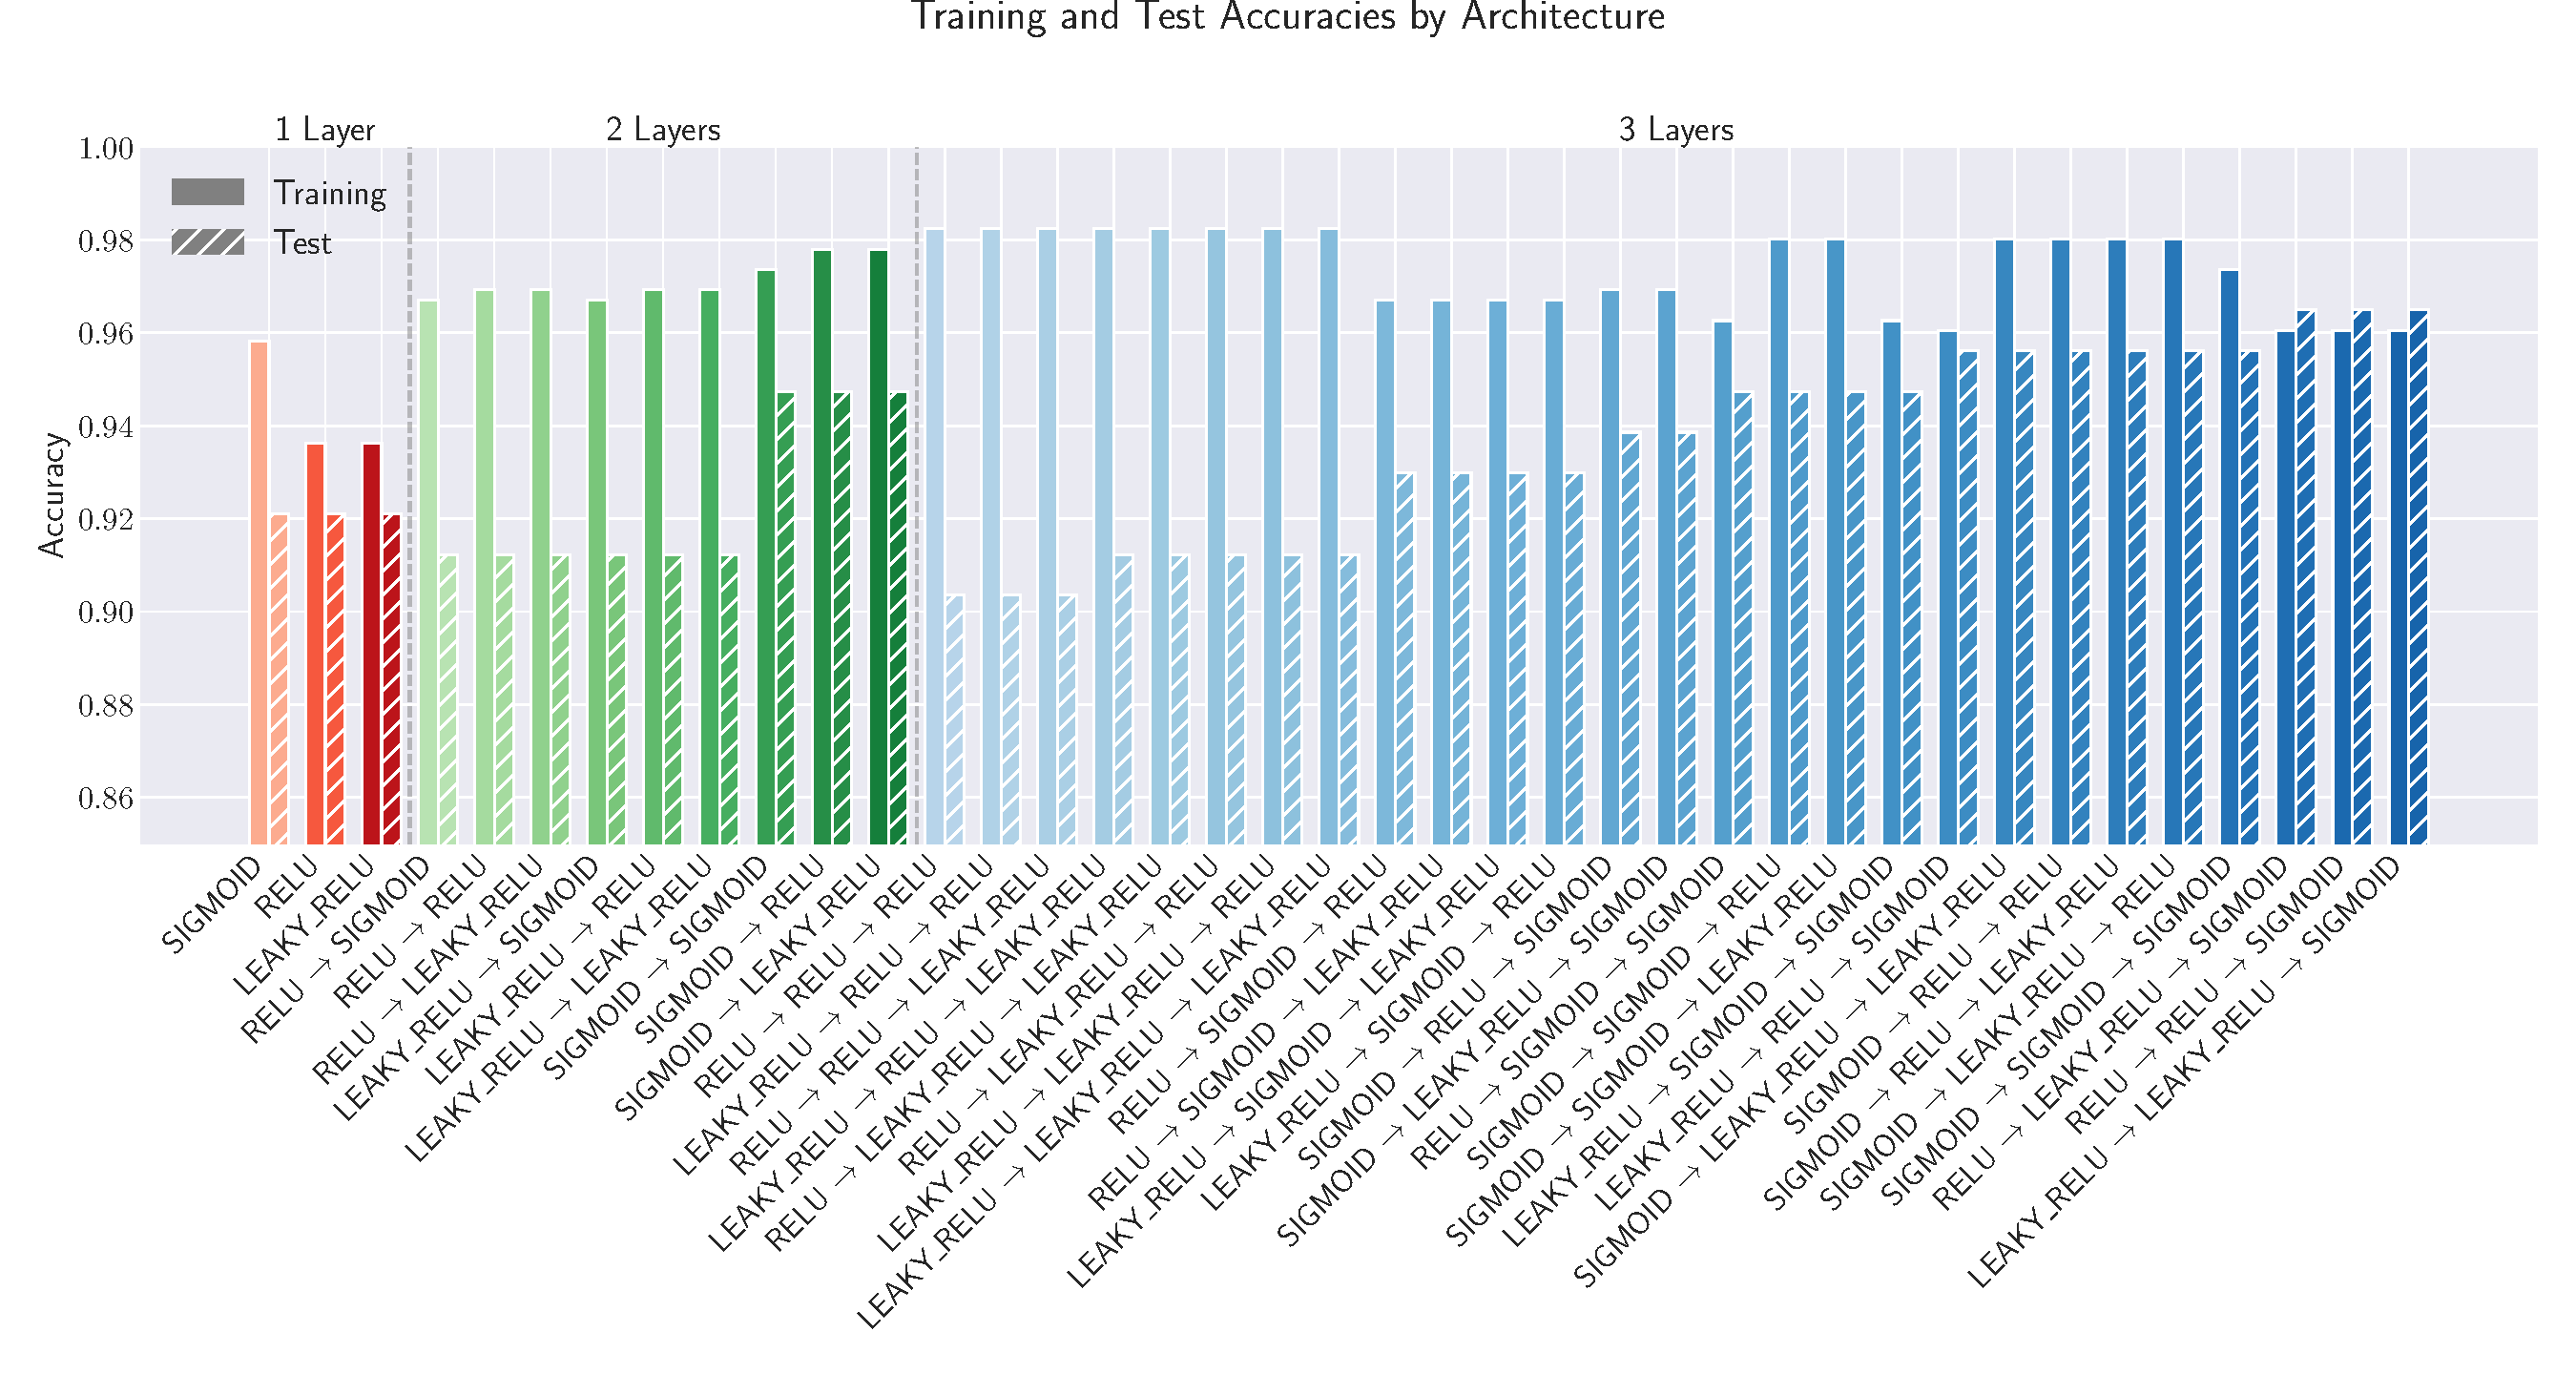
\includegraphics[width=1\textwidth]{../figs/classification_activations_layers_multi.pdf}
    \caption{The experiment from \cref{fig:NN_Classification_activations_layers} extended to allow for all combinations of activation functions through hidden layers 1-3.}
\end{figure}

\end{document}

% MAYBE REMOVE

% LINK WITH SPECIFIC NAME
% \href{https://raw.github.uio.no/oskarei/CompFys-Project5/main/data/gif/triple_slit_200_81_anim.gif?token=GHSAT0AAAAAAAAAIZKJAEIVBDMTTIDARGUYZMAXTHA}{triple-slit}

% MATHMODE IN HEADLINE
% \subsubsection{\texorpdfstring{$\text{Re}(u_{i,j}^n)$ and $\text{Im}(u_{i,j}^n)$}{Lg}}

% FIGURE COVERING BOTH COLUMNS
% \begin{figure*}
%   \vspace*{-5pt}
%   \centering %Centers the figure
%   \includegraphics[width=\textwidth]{../data/fig/triple_slit.pdf}
%   \caption{The square root of the probabilities at each point in the box $\sqrt{p_{i,j}^n}$ at the beginning (top left), middle (top center) and end (top right) of the triple-slit simulation with adjusted initialization and potential position. The plot at the bottom shows the normalized probability values $p(y\:|\:x=0.9;\;t=0.0025)$ along the detection screen at $x = 0.9$ at the end of the simulation.}\label{fig:TripleSlit}
%   \vspace*{-5pt}
% \end{figure*}

% FIGURE IN SINGLE COLUMN
% \begin{figure}[h!]
%   %\vspace*{-5pt}
%   \centering %Centers the figure
%   \includegraphics[width=0.9\columnwidth]{../data/fig/triple_sketch.png}
%   \caption{Illustration showing how the triple-slit interference pattern changes with distance from the slits. Gathered from Physics StackExchange \cite{TripleSketch}.}\label{fig:TripleSketch}
%   \vspace*{-10pt}
% \end{figure}

% TABLE COVERING BOTH COLUMNS
% \begin{center}
%   \vspace{-10pt}
%   \renewcommand{\arraystretch}{1.5}
%   \begin{table*}
%   %\centering
%   \begin{tabular}{| C{3.5cm} | C{2.2cm} | C{2.2cm} |  C{2.2cm} |  C{2.2cm} |  C{2.2cm} |  C{2.2cm} |}
%   \hline
%   \hspace{1pt} & \textbf{Model \hyperref[fig:potential model A]{A}} & \textbf{Model \hyperref[fig:potential model B]{B}} & \textbf{Model \hyperref[fig:potential model C]{C}} & \textbf{Model \hyperref[fig:potential model D]{D}} & \textbf{Model \hyperref[fig:potential model E]{E}} & \textbf{Model \hyperref[fig:potential model F]{F}} \\
%   \hline
%   \boldmath$m_0/M_{\astrosun}$ & $0.95$ & $0.95$ & $1.00$ & $1.00$ & $1.00$ & $1.05$ \\
%   \hline
%   \boldmath$r_0/R_{\astrosun}$ & $1.00$ & $1.25$ & $1.00$ & $1.00$ & $1.00$ & $1.50$ \\
%   \hline
%   \boldmath$L_0/L_{\astrosun}$ & $1.25$ & $1.00$ & $1.25$ & $1.50$ & $1.50$ & $1.00$ \\
%   \hline
%   \boldmath$\rho_0/\overline{\rho}_{\astrosun}$ & $1.00\times10^{-5}$ & $1.00\times10^{-5}$ & $7.50\times10^{-6}$ & $1.00\times10^{-5}$ & $2.50\times10^{-5}$ & $1.25\times10^{-5}$ \\
%   \hline
%   \textbf{Reach of }\boldmath{$m/m_0$} & $3.02\:\%$ & $4.24\:\%$ & $1.18\:\%$ & $2.66\:\%$ & $4.40\:\%$ & $3.79\:\%$ \\
%   \hline
%   \textbf{Reach of }\boldmath{$r/r_0$} & $0.73\:\%$ & $0.34\:\%$ & $0.06\:\%$ & $0.39\:\%$ & $0.51\:\%$ & $0.19\:\%$ \\
%   \hline
%   \textbf{Reach of }\boldmath{$L/L_0$} & $0.03\:\%$ & $0.14\:\%$ & $0.08\:\%$ & $0.04\:\%$ & $0.11\:\%$ & $0.21\:\%$ \\
%   \hline
%   \textbf{Size of core} & $0.24\times r_0$ & $0.19\times r_0$ & $0.26\times r_0$ & $0.25\times r_0$  & $0.24\times r_0$  & $0.15\times r_0$ \\
%   \hline
%   \textbf{Width of main zone} & $0.21\times r_0$ & $0.24\times r_0$ & $0.17\times r_0$ & $0.21\times r_0$ & $0.30\times r_0$ & $0.28\times r_0$ \\
%   \hline
%   \boldmath$F_\textbf{small}/F_\textbf{main}$ & No zone & No zone & $8.39\:\%$ & No zone & No zone & No zone \\
%   \hline
%   \end{tabular}
%   \cprotect\caption{The first four rows contain the initial mass, radius, luminosity and mass density of the six models, respectively. The initial temperature was $T_0 = 5770\:\text{K}$ for all six models, and the initial pressure was decided by the initial mass density through the equation of state. The next three rows show how far $m$, $r$ and $L$ reached before the integration was stopped, respectively. The size of the core and of the main convection zone near the surface, both given in units of $r_0$, are listed in the two next rows. In the last row I have listed the ratios between the convective flux from an eventual second, smaller convection zone and the convective flux from the respective main convection zone. If it says ``No zone'', the model does not have any more convection zones.}\label{tab:models}
%   \end{table*}
%   \renewcommand{\arraystretch}{1}
%   \vspace{-20pt}
% \end{center}

% STANDARD TABLE IN SINGLE COLUMN
% \begin{center}
%   \renewcommand{\arraystretch}{1.5}
%   \begin{table}[h!]
%   \centering
%   \begin{tabular}{| C{2.2cm} | C{1.4cm} | C{1.4cm} | C{1.4cm} | C{1.4cm} |}
%   \hline
%   \textbf{No. of cycles} & \boldmath$\left<ϵ\right>$ \boldmath$[J]$ & \boldmath$\left<|m|\right>$ & \boldmath$C_V$ \boldmath$[k_\text{B}]$ & \boldmath$\chi$ \boldmath$[J^{-1}]$ \\
%   \hline
%   10 & $-1.8000$ & 0.9375 & 1.4400 & 0.1594 \\
%   \hline
%   20 & $-1.9000$ & 0.9688 & 0.7600 & 0.0836 \\
%   \hline
%   50 & $-1.9600$ & 0.9875 & 0.3136 & 0.0344 \\
%   \hline
%   100 & $-1.9800$ & 0.9938 & 0.1584 & 0.0173 \\
%   \hline
%   200 & $-1.9775$ & 0.9931 & 0.1780 & 0.0186 \\
%   \hline
%   500 & $-1.9880$ & 0.9962 & 0.0954 & 0.0104 \\
%   \hline
%   1000 & $-1.9940$ & 0.9981 & 0.0479 & 0.0052 \\
%   \hline
%   5000 & $-1.9960$ & 0.9988 & 0.0319 & 0.0033 \\
%   \hline
%   10000 & $-1.9974$ & 0.9992 & 0.0204 & 0.0022 \\
%   \hline
%   100000 & $-1.9975$ & 0.9992 & 0.0197 & 0.0022 \\
%   \hline
%   1000000 & $-1.9973$ & 0.9992 & 0.0215 & 0.0023 \\
%   \hline
%   \textbf{Analytical} & $-1.9960$ & 0.9987 & 0.0321 & 0.0040 \\
%   \hline
%   \end{tabular}
%   \cprotect\caption{Numerical estimates of $\left<\epsilon\right>$, $\left<|m|\right>$, $C_V$ and $\chi$ for $T = 1.0\:J/k_\text{B}$ after increasing numbers of Monte Carlo cycles are performed. The last row contains the analytical values.}\label{tab:2x2 results}
%   \end{table}
%   \renewcommand{\arraystretch}{1}
% \end{center}

% TABLE WITH MULTIROW
% \begin{center}
%   \renewcommand{\arraystretch}{1.5}
%   \begin{table}[h!]
%   \centering
%   \begin{tabular}{| C{2.4cm} | C{1.5cm} | C{1.1cm} | C{2.0cm} |}
%   \hline
%   \textbf{No. of} \boldmath$s = +1$ & \boldmath$E(\mathbf{s})$ \boldmath$[J]$ & \boldmath$M(\mathbf{s})$ & \textbf{Degeneracy} \\
%   \hline
%   0 & $-8$ & $-4$ & None \\
%   \hline
%   1 & \hspace{7pt}$0$ & $-2$ & $4$ \\
%   \hline
%   \multirow{2}{*}{2} & \hspace{7pt}$8$ & \multirow{2}{*}{\hspace{7pt}$0$} & $2$ \\
%   \cline{2-2}\cline{4-4}
%   & \hspace{7pt}$0$ & & $4$ \\
%   \hline
%   3 & \hspace{7pt}$0$ & \hspace{7pt}$2$ & $4$ \\
%   \hline
%   4 & $-8$ & \hspace{7pt}$4$ & None \\
%   \hline
%   \end{tabular}
%   \cprotect\caption{Total energy $E(\mathbf{s})$ and magnetisation $M(\mathbf{s})$ for a \texorpdfstring{$2\times2$}{Lg} lattice with $0$, $1$, $2$, $3$ and $4$ spins $s = +1$. Because we use periodic boundary conditions, the total energy can either be 0$\:J$ or 8$\:J$ when we have two spins $s = +1$ and two spins $s = -1$, depending on if the equal spins are neighbours or not. The last column contains the degeneracy level for the different combinations of number of spins $s = +1$ and total energy.}\label{tab:2x2 lattice}
%   \end{table}
%   \renewcommand{\arraystretch}{1}
% \end{center}

% ALGORITHM
% \begin{figure}
%   % NOTE: We only need \begin{figure} ... \end{figure} here because of a compatability issue between the 'revtex4-1' document class and the 'algorithm' environment.
%       \begin{algorithm}[H]
%       \caption{The Metropolis Algorithm}
%       \label{algo:Euler}
%           \begin{algorithmic}
%               \Procedure{Monte Carlo cycle}{$\mathbf{s}, L, β$}
%               \For{$i = 0, 1, \ldots, L-1$}
%               \For{$j = 0, 1, \ldots, L-1$}
%               \State $\triangleright$ Compute energy difference due to flipping $s_{ij}$
%               \State $\Delta E ← \Delta E_\text{function}(\mathbf{s}, i, j)$
%               \State
%               \State $\triangleright$ Flip if energy difference is negative or zero
%               \If{$\Delta E \leq 0$}
%                   \State $s_{ij} = -s_{ij}$ \Comment{Flip spin}
%                   \State
%               \Else \Comment{Energy difference is positive}
%                   \State $w = e^{-β\Delta E}$ \Comment{Probability of flipping spin}
%                   \State $\triangleright$ Generate random number $r ∈ [0,1]$
%                   \State $\triangleright$ Flip spin if $r≤ w$
%                   \If{$r≤ w$}
%                       \State $s_{ij} = -s_{ij}$ \Comment{Flip spin}
%                   \EndIf
%               \EndIf
%               \State
%               \State $\triangleright$ Calculate $E$, $E^2$, $|M|$ and $M^2$ for $\mathbf{s}$
%               \State $E$, $E^2 = E_\text{function}(\mathbf{s})$
%               \State $|M|$, $M^2 = M_\text{function}(\mathbf{s})$
%               \State $\triangleright$ Update expectation values accordingly
%               \EndFor
%               \EndFor
%               \EndProcedure
%           \end{algorithmic}
%       \end{algorithm}
%   \end{figure}
